\pdfminorversion=7
\documentclass[aspectratio=169,11pt]{beamer}

\IfFileExists{beamerthemeCCM.sty}{%
  \usetheme{CCM}
}{%
  \usetheme{default}
  \definecolor{CCMorange}{HTML}{F6862D}
  \definecolor{SFdark}{HTML}{1D2954}
  \definecolor{mygray}{HTML}{8F8F8F}
  \setbeamertemplate{navigation symbols}{}
  \setbeamertemplate{footline}[frame number]
  \setbeamersize{text margin left=0.25in,text margin right=0.25in}
  \setbeamercolor{title}{fg=CCMorange}
  \setbeamercolor{frametitle}{fg=CCMorange,bg=white}
  \setbeamercolor{item}{fg=CCMorange}
  \setbeamercolor{block title}{fg=black,bg=CCMorange!30}
  \setbeamercolor{block body}{fg=black,bg=black!3}
}

\usepackage{amsmath,amssymb,mathtools,mathrsfs}
\usepackage{bm}
\usepackage{booktabs}
\usepackage{graphicx}
\usepackage{times}
\usepackage{tikz}
\usetikzlibrary{arrows.meta,calc,positioning,decorations.pathreplacing}

\graphicspath{{day4_morning_figures/}}

\newcommand{\R}{\mathbb{R}}
\newcommand{\C}{\mathbb{C}}
\newcommand{\cO}{\mathcal{O}}
\newcommand{\dd}{\,\mathrm d}
\newcommand{\ii}{\mathrm i}
\newcommand{\x}{\bm{x}}
\newcommand{\y}{\bm{y}}
\newcommand{\s}{\bm{s}}
\newcommand{\rvec}{\bm{r}}
\newcommand{\nuvec}{\bm{\nu}}
% Shared operator notation for the AMSS FIEM talk slides.
% Change this one line to change the font for layer and volume potentials.
\newcommand{\FIEMopfont}[1]{\mathcal{#1}}

\newcommand{\Sop}{\FIEMopfont{S}}
\newcommand{\Dop}{\FIEMopfont{D}}
\newcommand{\Spop}{\Sop^{\prime}}
\newcommand{\Dpop}{\Dop^{\prime}}
\newcommand{\Vop}{\FIEMopfont{V}}
\newcommand{\Iop}{\FIEMopfont{I}}
\newcommand{\Kop}{\FIEMopfont{K}}
\newcommand{\KopT}{\Kop^{\prime}}
\newcommand{\Wop}{\FIEMopfont{W}}
\newcommand{\Aop}{\FIEMopfont{A}}
\newcommand{\Top}{\FIEMopfont{T}}

\newcommand{\hl}[1]{{\color{CCMorange}\textbf{#1}}}
\DeclareMathOperator{\rect}{rect}
\DeclareMathOperator{\erf}{erf}
\DeclareMathOperator{\Ei}{Ei}

\title{Day 4 Morning: Truncated Kernels and Function Extension}
\subtitle{FFT volume potentials and high-order solvers on complex domains}
\author{Fast Algorithms and Integral Equation Methods}
\institute{AMSS Summer Course}
\date{July 2026}

\setlength{\emergencystretch}{3em}

\begin{document}

%================================================================
\begin{frame}
  \titlepage
\end{frame}

%================================================================
\begin{frame}{TKM and function extension roadmap}
\small
\begin{columns}[T,totalwidth=\textwidth]
\begin{column}{0.48\textwidth}
\textbf{Part I: truncated kernel method (TKM)}
\begin{itemize}
  \item Free-space volume potentials.
  \item Why the FFT is not automatically a free-space solver.
  \item Physical-space truncation of Green's functions.
  \item Smooth spectral multipliers and standard FFTs.
  \item Matrix entries, derivatives, and volume integral equations.
\end{itemize}
\end{column}
\begin{column}{0.48\textwidth}
\textbf{Part II: Function Extension}
\begin{itemize}
  \item Why complex-domain data must be smoothly extended to a box.
  \item Finite Seeley-type formula along normals.
  \item Chebyshev nodes and explicit extension weights.
  \item Windowing and implementation on complex domains.
  \item Coupling FFT particular solutions with boundary-integral-equation (BIE) corrections.
\end{itemize}
\end{column}
\end{columns}
\end{frame}

%================================================================
\begin{frame}{Free-space convolution and smooth extension}
\small
The syllabus topic is:
\[
  \text{volume integrals and fast Poisson solvers.}
\]
The numerical decomposition uses two tools:
\[
  \boxed{\text{fast free-space convolution}}
  \quad+\quad
  \boxed{\text{smooth extension from complex domains to boxes}}.
\]

\begin{block}{Problem}
Free-space Green's functions are singular, and source data specified on a
complex domain must be extended smoothly before sampling it on an FFT box.
\end{block}

\begin{block}{Computational objective}
Build high-order particular solutions by FFT, then use boundary integral
equations only for the homogeneous boundary correction.
\end{block}
\end{frame}

%================================================================
\section{Truncated Kernel Method}

\begin{frame}{TKM objectives}
\small
The main mathematical and algorithmic objectives are:
\begin{enumerate}
  \item explain why naive FFT convolution gives a periodic problem;
  \item write the free-space volume potential as a convolution;
  \item state the physical-space truncation mechanism;
  \item derive the 3D Laplace truncated spectral multiplier;
  \item describe the FFT algorithm and its zero-padding requirements;
  \item explain the Nystr\"om matrix interpretation.
\end{enumerate}
\end{frame}

%================================================================
\begin{frame}{Volume potentials}
\small
Let $G$ be a free-space Green's function and let $f$ be supported in a box $D$.
The volume potential is
\[
  u(\x)=\int_D G(\x-\y)f(\y)\dd\y.
\]

\begin{itemize}
  \item $G$ is translation invariant.
  \item $G$ is usually singular at the origin.
  \item $G$ is long range.
  \item The source density is sampled on a uniform tensor grid.
\end{itemize}

\begin{block}{Numerical contract}
Given samples of $f$, compute samples of $u$ on the same box as if the
surrounding space were infinite, not periodic.
\end{block}
\end{frame}

%================================================================
\begin{frame}{Examples of Green's functions}
\small
Let $r=|\rvec|$. The conventions are
\[
  -\Delta G_0=\delta,\qquad
  (\Delta+k^2)G_k=-\delta,\qquad
  -\Delta^2G_b=\delta.
\]
\begin{columns}[T,totalwidth=\textwidth]
\begin{column}{0.48\textwidth}
\textbf{Three dimensions}
\[
  G_0(r)=\frac{1}{4\pi r},
  \qquad
  G_k(r)=\frac{e^{ikr}}{4\pi r}.
\]
\[
  G_b(r)=\frac{r}{8\pi}
  \quad\text{for the biharmonic equation.}
\]
\end{column}
\begin{column}{0.48\textwidth}
\textbf{Two dimensions}
\[
  G_0(r)=-\frac{1}{2\pi}\log r,
  \qquad
  G_k(r)=\frac{\ii}{4}H_0^{(1)}(kr).
\]
\[
  G_b(r)=-\frac{r^2}{8\pi}(\log r-1).
\]
\end{column}
\end{columns}
\end{frame}

%================================================================
\begin{frame}{Direct summation complexity}
\small
On an $N^d$ grid, a direct volume convolution costs
\[
  \cO(N^{2d})
\]
operations.

\vspace{2mm}
\begin{block}{Desired complexity}
For smooth data on a uniform grid, the algorithmic complexity should be
\[
  \cO(N^d\log N)
\]
using the standard FFT.
\end{block}
\end{frame}

%================================================================
\begin{frame}{FFT acceleration and its limitation}
\small
The convolution theorem says
\[
  u=G*f
  \quad\Longrightarrow\quad
  \widehat{u}(\s)=\widehat{G}(\s)\widehat{f}(\s).
\]

\begin{itemize}
  \item Compute $\widehat{f}$ with an FFT.
  \item Multiply by a spectral Green's function.
  \item Inverse FFT back to physical space.
\end{itemize}

\vspace{2mm}
Two limitations must be addressed: periodicity and singular spectral
multipliers.
\end{frame}

%================================================================
\begin{frame}{The periodicity problem}
\small
An FFT on a finite box computes a periodic convolution unless we prevent wrap-around.
\[
  \sum_{\y\in D}G(\x-\y)f(\y)
  \quad\leadsto\quad
  \sum_{\y\in D}\sum_{m\in\mathbb{Z}^d}
  G(\x-\y+mP)f(\y).
\]

\begin{itemize}
  \item Periodic images are not part of the free-space solution.
  \item Zero padding removes wrap-around for compactly supported discrete kernels.
  \item Free-space Green's functions are not compactly supported.
\end{itemize}
\end{frame}

%================================================================
\begin{frame}{Aperiodic convolution and padding}
\small
For a discrete convolution on a box, the FFT computes
\[
  u_i^{\rm FFT}
  =
  \sum_j \sum_{m\in\mathbb Z^d}
  T_{i-j+mM} f_j .
\]
For a compact discrete stencil, choose the padding so that circular shifts do
not overlap the source and target entries of interest. The factor-two embedding
for a square aperiodic convolution is derived below in matrix form.

\vspace{1mm}
TKM makes this argument valid for Green's functions by replacing the infinite
kernel with a compactly supported kernel $G^L$.  The padding condition is then
a geometric support condition, not a heuristic.
\end{frame}

%================================================================
\begin{frame}{The spectral singularity problem}
\small
For Poisson in free space,
\[
  -\Delta u=f
  \quad\Longrightarrow\quad
  \widehat{u}(\s)=\frac{\widehat{f}(\s)}{|\s|^2}
\]
for the Fourier transform convention used here.

\vspace{2mm}
For Helmholtz,
\[
  \widehat{u}(\s)=\frac{\widehat{f}(\s)}{|\s|^2-k^2}.
\]

\begin{itemize}
  \item Poisson has a singularity at $\s=0$.
  \item Helmholtz has a singularity on the sphere $|\s|=k$.
  \item A tensor-product trapezoidal rule does not like these singular sets.
\end{itemize}
\end{frame}

%================================================================
\begin{frame}{Classical FFT workarounds}
\small
\textbf{Local correction in physical space}
\[
  \text{FFT convolution with sampled }G
  +
  \text{corrected weights near }r=0.
\]
This can be high order but requires kernel-specific corrected weights.

\vspace{3mm}
\textbf{Special quadrature in Fourier space}
\[
  \int e^{\ii \s\cdot\x}
  \frac{\widehat f(\s)}{|\s|^2-k^2}\dd\s.
\]
This can be high order but becomes technical when the singular set is complicated.
\end{frame}

%================================================================
\begin{frame}{Truncated kernel method}
\small
Replace the Green's function by a truncated Green's function:
\[
  G^L(\rvec)=G(\rvec)\rect\!\left(\frac{|\rvec|}{2L}\right).
\]
Here $\rect(t)=1$ for $|t|<\tfrac12$ and $\rect(t)=0$ for $|t|>\tfrac12$.
Thus $G^L(\rvec)=G(\rvec)$ for $|\rvec|<L$ and vanishes for $|\rvec|>L$.

\vspace{1mm}
Choose $L$ larger than every source-target distance of interest. Then, for
each target $\x\in D$,
\[
  \int_D G(\x-\y)f(\y)\dd\y
  =
  \int_D G^L(\x-\y)f(\y)\dd\y
\]

The physical-space interactions are unchanged, while the truncated multiplier
is smooth and can be sampled on a Cartesian frequency grid.
\end{frame}

%================================================================
\begin{frame}{Choosing the truncation radius}
\small
If the target and source are both in a unit box in $\R^d$, then
\[
  |\x-\y|\le \sqrt d.
\]
It is enough to choose
\[
  L>\sqrt d.
\]

\vspace{2mm}
More generally:
\[
  L>\max_{\x\in X,\ \y\in Y}|\x-\y|.
\]
\begin{itemize}
  \item Larger $L$ is safe but increases spectral oscillation.
  \item Smaller $L$ aliases the intended free-space interaction.
\end{itemize}
\end{frame}

%================================================================
\begin{frame}{Truncation and the Fourier multiplier}
\small
The truncated kernel is compactly supported:
\[
  G^L(\rvec)=0,\qquad |\rvec|>L.
\]
By Paley-Wiener theory, its Fourier transform is entire:
\[
  \widehat{G^L}(\s)=\mathscr{F}[G^L](\s)
  \quad\text{is smooth for all }\s.
\]

\begin{block}{Numerical consequence}
The inverse Fourier integral can now be sampled by the trapezoidal rule on a Cartesian grid and evaluated by FFT.
\end{block}
\end{frame}

%================================================================
\begin{frame}{Radial Fourier transform in 3D}
\small
For a radial function $f(r)$ in $\R^3$,
\[
  F(s)=4\pi\int_0^\infty
  \frac{\sin(sr)}{sr}f(r)r^2\dd r,
  \qquad s=|\s|.
\]

\vspace{2mm}
This turns a 3D Fourier transform of a radial kernel into a one-dimensional integral.
\end{frame}

%================================================================
\begin{frame}{Derivation: 3D Laplace truncated kernel}
\small
Use
\[
  G_0^L(r)=\frac{1}{4\pi r}\rect\left(\frac{r}{2L}\right).
\]
Then
\[
\begin{aligned}
  \widehat{G_0^L}(s)
  &=4\pi\int_0^L
  \frac{\sin(sr)}{sr}\frac{1}{4\pi r}r^2\dd r \\
  &=\int_0^L\frac{\sin(sr)}{s}\dd r
  =\frac{1-\cos(Ls)}{s^2}.
\end{aligned}
\]
Equivalently,
\[
  \widehat{G_0^L}(s)=2\left(\frac{\sin(Ls/2)}{s}\right)^2.
\]
\end{frame}

%================================================================
\begin{frame}{The singularity is removable}
\small
Although the formula contains $s$ in the denominator,
\[
  \widehat{G_0^L}(s)=2\left(\frac{\sin(Ls/2)}{s}\right)^2
\]
has a finite limit at $s=0$:
\[
  \widehat{G_0^L}(0)=\frac{L^2}{2}.
\]

\begin{itemize}
  \item The original free-space multiplier is singular.
  \item The truncated multiplier is analytic.
  \item In code, use a series expansion near $s=0$.
\end{itemize}
\end{frame}

%================================================================
\begin{frame}{The resulting Poisson formula}
\small
For the 3D Poisson volume potential,
\[
  u(\x)=\int_D\frac{f(\y)}{4\pi|\x-\y|}\dd\y,
\]
we compute
\[
  u(\x)=
  \frac{1}{(2\pi)^3}
  \int_{\R^3}
  e^{\ii\s\cdot\x}
  \widehat{G_0^L}(\s)\widehat{f}(\s)\dd\s,
\]
where
\[
  \widehat{G_0^L}(\s)=2\left(\frac{\sin(L|\s|/2)}{|\s|}\right)^2.
\]
\end{frame}

%================================================================
\begin{frame}{Radial Fourier transform in 2D}
\small
For a radial function $f(r)$ in $\R^2$,
\[
  F(s)=2\pi\int_0^\infty J_0(sr)f(r)r\dd r.
\]

For the 2D Laplace kernel,
\[
  G_0(r)=-\frac{1}{2\pi}\log r,
\]
the truncated spectral multiplier is
\[
  \widehat{G_0^L}(s)=
  \frac{1-J_0(Ls)}{s^2}
  -
  \frac{L\log(L)J_1(Ls)}{s}.
\]
\end{frame}

%================================================================
\begin{frame}{3D Helmholtz multiplier}
\small
For
\[
  G_k(r)=\frac{e^{ikr}}{4\pi r},
\]
the truncated 3D Helmholtz multiplier is
\[
  \widehat{G_k^L}(s)=
  \frac{-1+e^{\ii Lk}\left(\cos(Ls)-\ii\frac{k}{s}\sin(Ls)\right)}
       {(k-s)(k+s)}.
\]

\begin{itemize}
  \item The apparent singularity at $s=k$ is removable.
  \item This is much easier to sample than the original distributional multiplier.
\end{itemize}
\end{frame}

%================================================================
\begin{frame}{2D Helmholtz multiplier}
\small
For
\[
  G_k(r)=\frac{\ii}{4}H_0^{(1)}(kr),
\]
the truncated 2D multiplier can be written using Bessel and Hankel functions:
\[
  \widehat{G_k^L}(s)=
  \frac{1+\frac{\ii\pi}{2}LsJ_1(Ls)H_0^{(1)}(Lk)
  -\frac{\ii\pi}{2}LkJ_0(Ls)H_1^{(1)}(Lk)}
  {s^2-k^2}.
\]

\vspace{2mm}
Again, the pole is removable after truncation.
\end{frame}

%================================================================
\begin{frame}{Spectra before and after truncation}
\centering
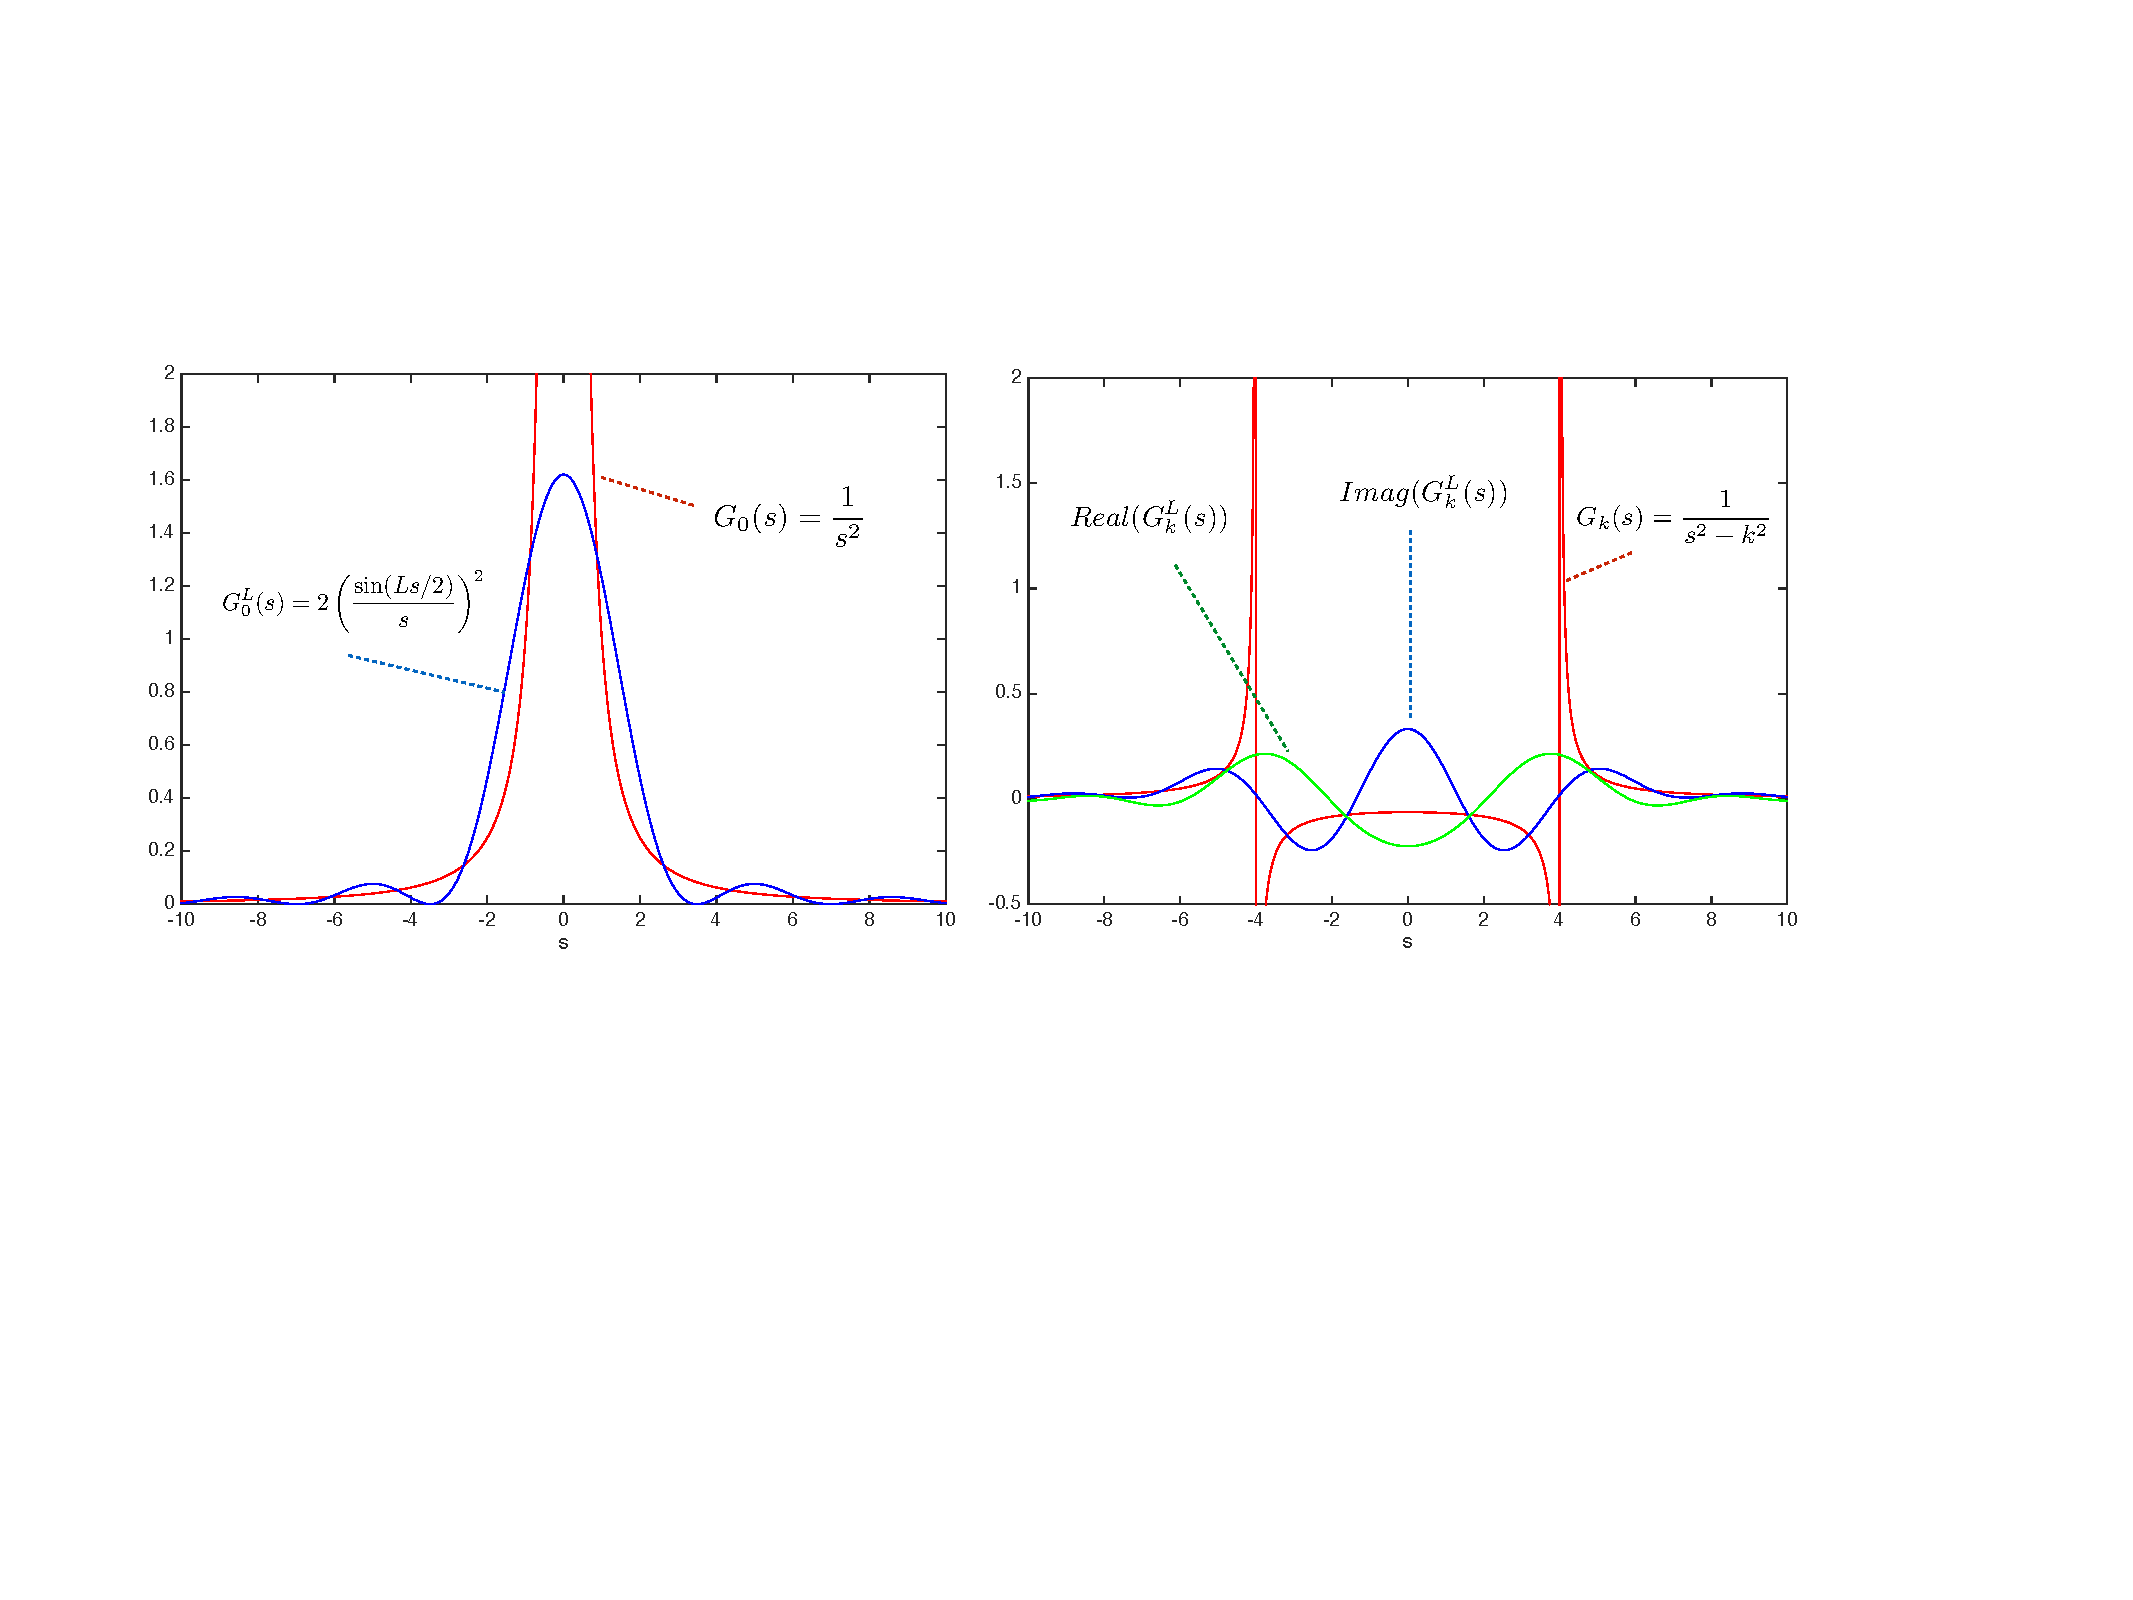
\includegraphics[width=0.90\textwidth,height=0.70\textheight,keepaspectratio]{figs12merge.pdf}

\vspace{1mm}
\scriptsize Free-space multipliers have singular behavior; truncated multipliers are smooth but oscillatory.
\end{frame}

%================================================================
\begin{frame}{Sampling requirement}
\small
The truncated multiplier is smooth, but it oscillates because the physical-space kernel has compact support.

\vspace{2mm}
For a unit box discretized with $N$ points per dimension, we use a grid of size
\[
  (4N)^d
\]
for the direct spectral construction of the stencil. The factor-two circulant
embedding used for subsequent applications is a separate step.
\end{frame}

%================================================================
\begin{frame}{Oscillation of the truncated multiplier}
\small
The 3D Laplace multiplier is
\[
  \widehat{G_0^L}(s)=\frac{1-\cos(Ls)}{s^2}.
\]
Its oscillation scale in frequency is
\[
  \Delta s\sim \frac{1}{L}.
\]
The inverse Fourier integral also contains
\[
  e^{\ii\s\cdot\x}\widehat f(\s),
\]
so the frequency grid must resolve both the source spectrum and the truncated
kernel spectrum.

\begin{block}{Tradeoff}
Choosing larger $L$ makes the physical truncation safer, but makes
$\widehat{G^L}$ more
oscillatory.  Choosing smaller $L$ makes the spectrum easier but risks changing
the actual free-space interaction.
\end{block}
\end{frame}

%================================================================
\begin{frame}{Direct TKM algorithm}
\small
\begin{enumerate}
  \item Zero-pad the source density to a sufficiently large box.
  \item Compute $\widehat f$ by FFT.
  \item Evaluate the smooth multiplier $\widehat{G^L}(\s)$ on the frequency grid.
  \item Multiply: $\widehat u(\s)=\widehat{G^L}(\s)\widehat f(\s)$.
  \item Inverse FFT.
  \item Restrict the result to the original target box.
\end{enumerate}

\vspace{2mm}
The method uses only trapezoidal quadrature and standard FFTs.
\end{frame}

%================================================================
\begin{frame}{Discrete Fourier quadrature formula}
\small
On a padded box of side length $P$ with even $M$ and spacing $h=P/M$, use
the multi-index $m=(m_1,\ldots,m_d)$ and frequencies
\[
  \s_m=\frac{2\pi}{P}m,\qquad
  m_\ell=-M/2,\ldots,M/2-1.
\]
The continuous formula is approximated by
\[
  u(\x_j)
  \approx
  \frac{(\Delta s)^d}{(2\pi)^d}
  \sum_m e^{\ii\s_m\cdot\x_j}
  \widehat{G^L}(\s_m)\widehat f(\s_m),
  \qquad
  \Delta s=\frac{2\pi}{P}.
\]
The source transform is approximated by
\[
  \widehat f(\s_m)\approx h^d\sum_n e^{-\ii\s_m\cdot\y_n}f_n.
\]

\vspace{1mm}
This is exactly the algebra implemented by FFTs once the data are placed on the
padded tensor grid.
\end{frame}

%================================================================
\begin{frame}{Superalgebraic convergence}
\small
If $f$ is smooth and compactly supported in the computational box, then $\widehat f$ decays rapidly.

\vspace{2mm}
Since $\widehat{G^L}$ is smooth,
\[
  \widehat{G^L}(\s)\widehat f(\s)
\]
also decays rapidly, and the trapezoidal approximation to the inverse Fourier integral converges superalgebraically.

\begin{block}{Where smoothness is used}
TKM is an FFT method for smooth volume data. If the density has jumps, the Fourier convergence is limited.
\end{block}
\end{frame}

%================================================================
\begin{frame}{Aperiodic convolution is a Toeplitz matrix product}
\small
For $N$ grid points in one coordinate, the stencil defines
\[
  \bm u=A\bm f,
  \qquad A_{ij}=T_{i-j},\qquad 0\le i,j<N.
\]
Thus the aperiodic convolution matrix is Toeplitz:
\[
  A=\begin{bmatrix}
  T_0&T_{-1}&\cdots&T_{-(N-1)}\\
  T_1&T_0&\ddots&\vdots\\
  \vdots&\ddots&\ddots&T_{-1}\\
  T_{N-1}&\cdots&T_1&T_0
  \end{bmatrix}.
\]
The entries required for one application have offsets
$-(N-1),\ldots,N-1$.  The next slide embeds this matrix in a circulant one.
\end{frame}

%================================================================
\begin{frame}{Factor-two padding gives a circulant embedding}
\small
Define the padded vector and the first column of a $2N\times2N$ circulant
matrix by
\[
  \widetilde{\bm f}=\begin{bmatrix}\bm f\\\bm{0}\end{bmatrix},
  \qquad
  \bm c^{\mathsf T}
  =
  \begin{bmatrix}
  T_0&T_1&\cdots&T_{N-1}&0&T_{-(N-1)}&\cdots&T_{-1}
  \end{bmatrix}.
\]
With $C=\operatorname{circ}(\bm c)$,
\[
  C\widetilde{\bm f}=
  \begin{bmatrix}A\bm f\\\bm r\end{bmatrix}.
\]
The lower block $\bm r$ is generally nonzero.  The desired Toeplitz product is
the restricted circulant product:
\[
  A=
  \begin{bmatrix}I&0\end{bmatrix}
  C
  \begin{bmatrix}I\\0\end{bmatrix}.
\]
\end{frame}

%================================================================
\begin{frame}{Why a circulant convolution is computed by FFT}
\small
Let $F_{2N}$ be the discrete Fourier transform matrix.  Every circulant matrix
is diagonalized by the Fourier basis:
\[
  F_{2N}CF_{2N}^{-1}=\operatorname{diag}(F_{2N}\bm c).
\]
Indeed, for the Fourier vector $v_j^{(m)}=e^{2\pi\ii mj/(2N)}$,
\[
  (Cv^{(m)})_i
  =\sum_j c_{(i-j)\bmod 2N}v_j^{(m)}
  =v_i^{(m)}\sum_\ell c_\ell e^{-2\pi\ii m\ell/(2N)}.
\]
Therefore one circulant convolution is evaluated as
\[
  C\widetilde{\bm f}
  =F_{2N}^{-1}\left[
    (F_{2N}\bm c)\odot(F_{2N}\widetilde{\bm f})
  \right].
\]
In $d$ dimensions, the tensor-product construction uses a $(2N)^d$ FFT grid.
\end{frame}

%================================================================
\begin{frame}{Precomputation: reduce from $4N$ to $2N$}
\small
The discrete operator is translation invariant:
\[
  u_{i'j'k'}=
  \sum_{i,j,k}
  T(i'-i,j'-j,k'-k)f_{ijk}.
\]

\vspace{2mm}
Compute the stencil $T$ once by applying the accurate $4N$ spectral construction to a discrete delta source.
Then subsequent applications use standard aperiodic convolution with zero padding by a factor of $2$.
\end{frame}

%================================================================
\begin{frame}{Nystr\"om interpretation}
\small
The precomputed stencil gives matrix entries for a high-order discretization:
\[
  A_{ij}=T(i-j).
\]

\begin{itemize}
  \item The singular self interaction is already regularized by the construction.
  \item All entries come from one accurate precomputation.
  \item The matrix can be used in iterative solvers, preconditioners, or direct solvers.
\end{itemize}
\end{frame}

%================================================================
\begin{frame}{Mollified Green's function entries}
\centering
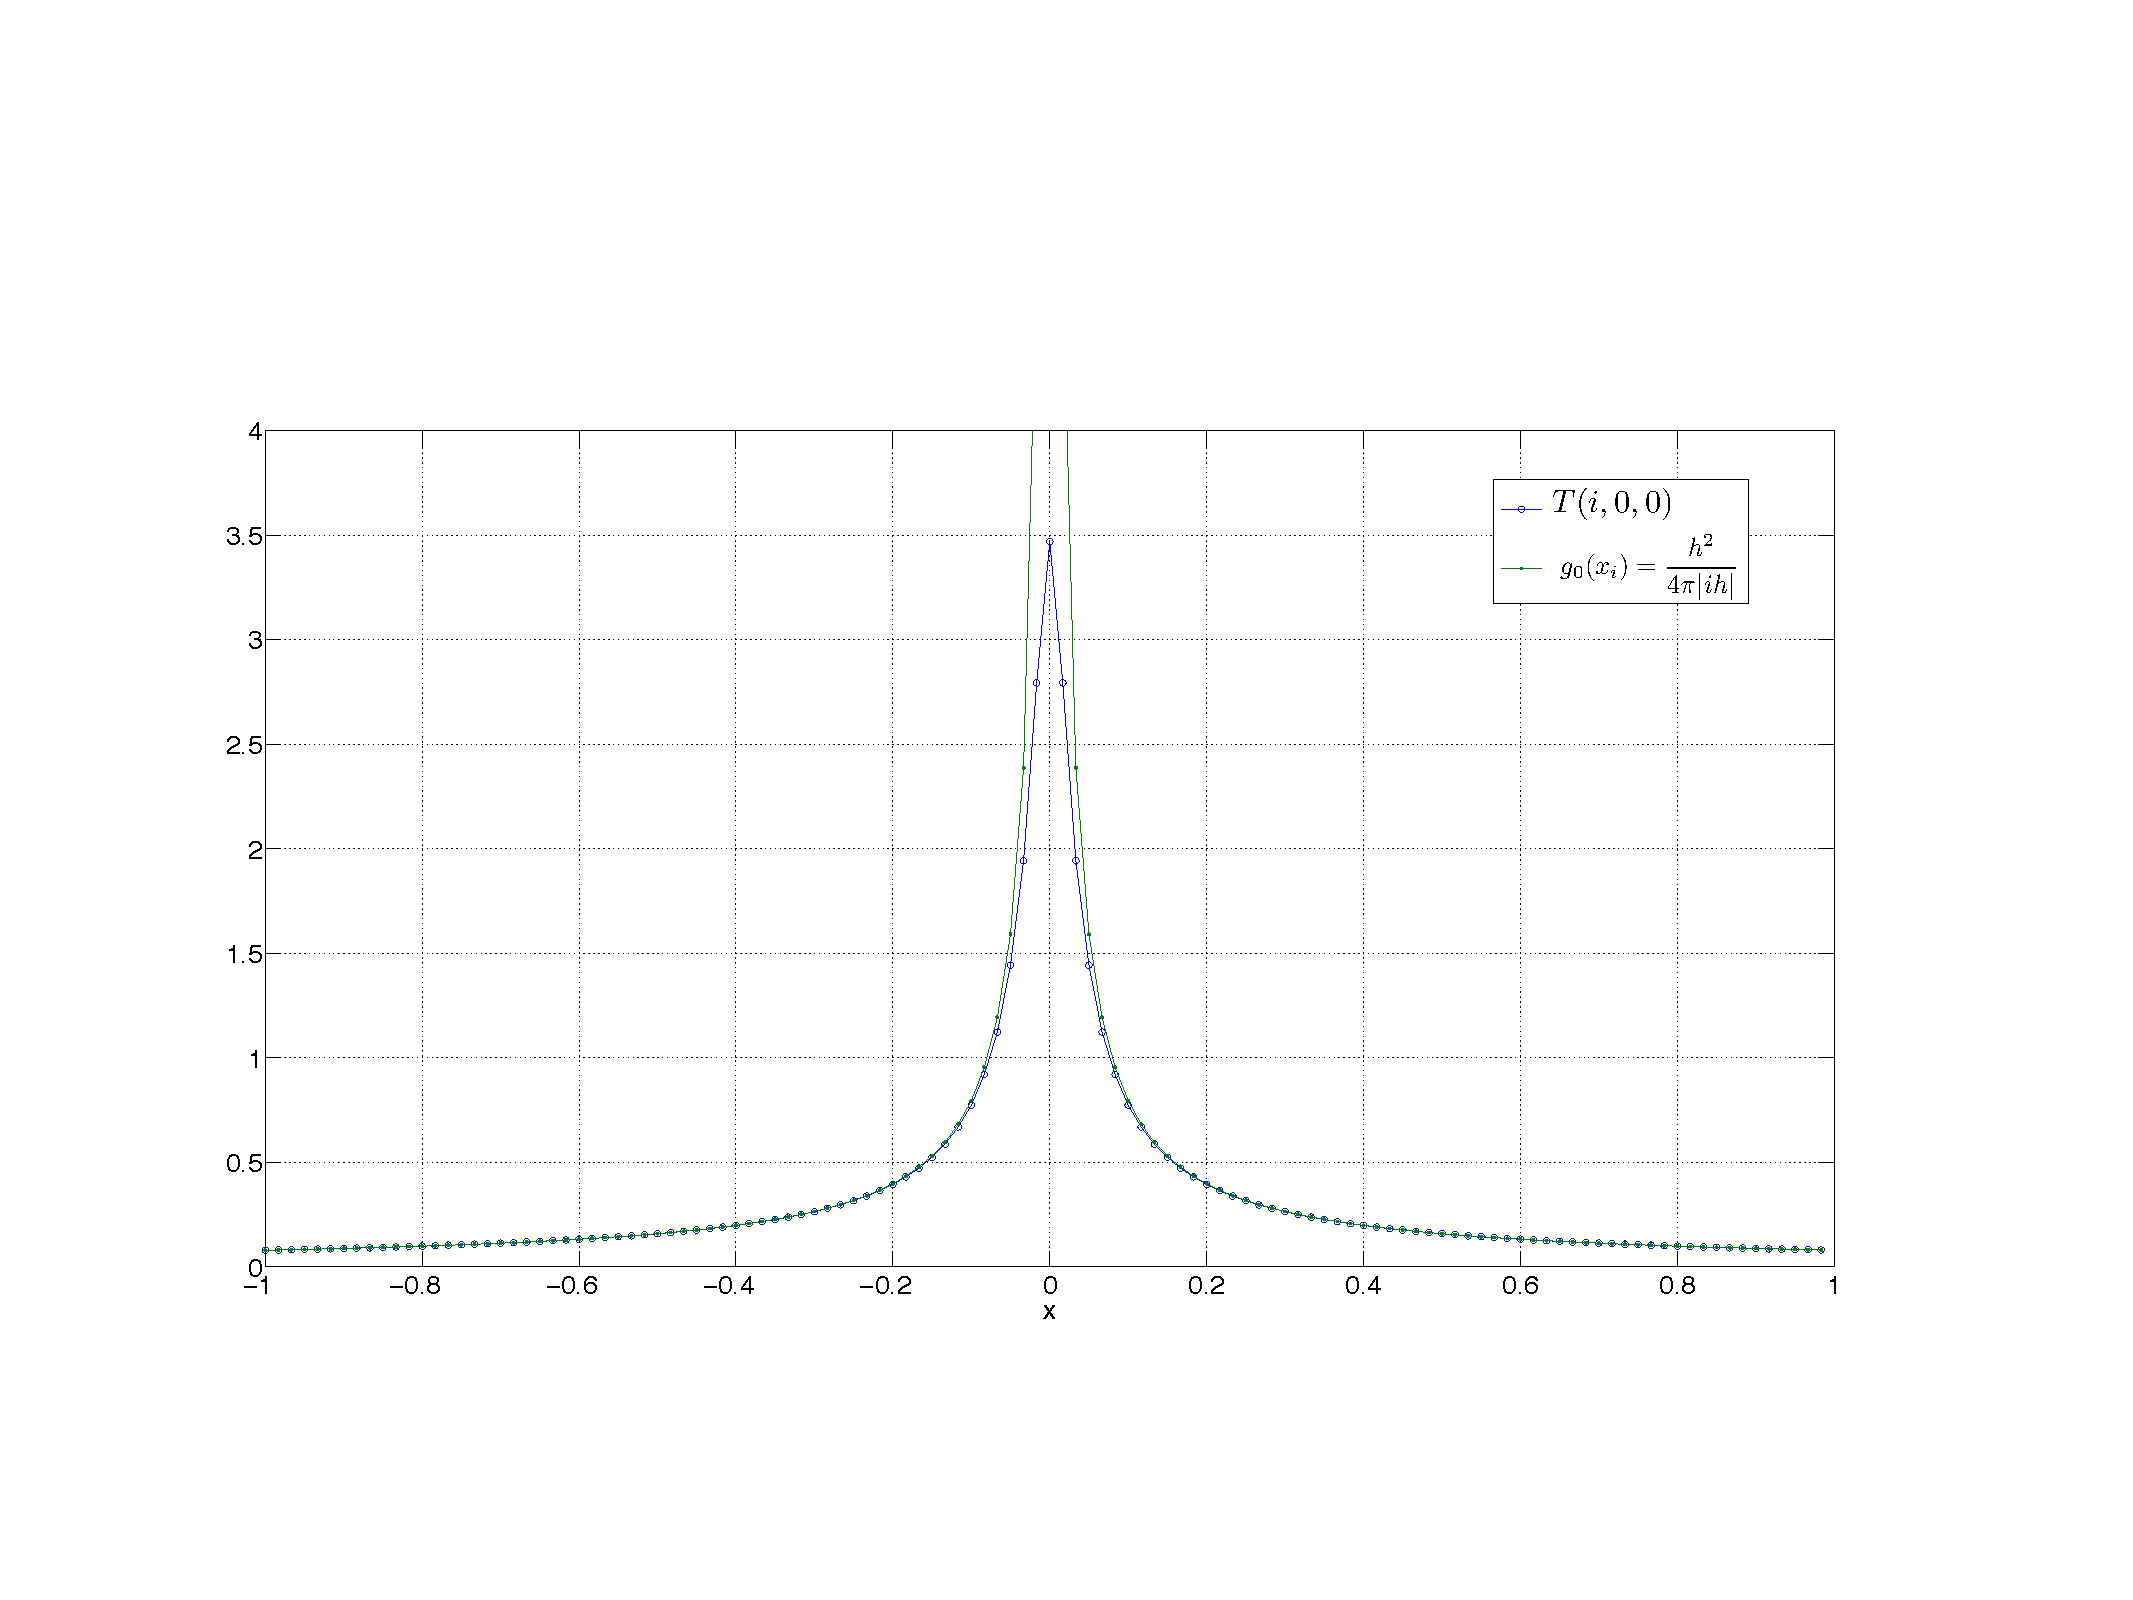
\includegraphics[height=0.72\textheight]{matrix_vs_g.pdf}

\vspace{1mm}
\scriptsize The precomputed high-order stencil behaves like a smooth, mollified Green's function near the singularity.
\end{frame}

%================================================================
\begin{frame}{Derivative evaluation by spectral multipliers}
\small
If
\[
  u=\mathscr{F}^{-1}\left[\widehat{G^L}(\s)\widehat f(\s)\right],
\]
then
\[
  \partial_{x_\ell}u
  =
  \mathscr{F}^{-1}\left[\ii s_\ell\widehat{G^L}(\s)\widehat f(\s)\right].
\]

\vspace{2mm}
Each derivative costs one additional inverse FFT after the source transform is known.
\end{frame}

%================================================================
\begin{frame}{Gaussian tests}
\small
For a Gaussian source in 3D,
\[
  \rho(r)=\frac{1}{\sigma^3(2\pi)^{3/2}}
  e^{-r^2/(2\sigma^2)}.
\]
The Poisson potential has the analytic form
\[
  (G_0*\rho)(\x)
  =
  \frac{1}{4\pi r}
  \erf\left(\frac{r}{\sqrt{2}\sigma}\right).
\]

\vspace{2mm}
This provides an analytic convergence test.
\end{frame}

%================================================================
\begin{frame}{Convergence for model kernels}
\centering
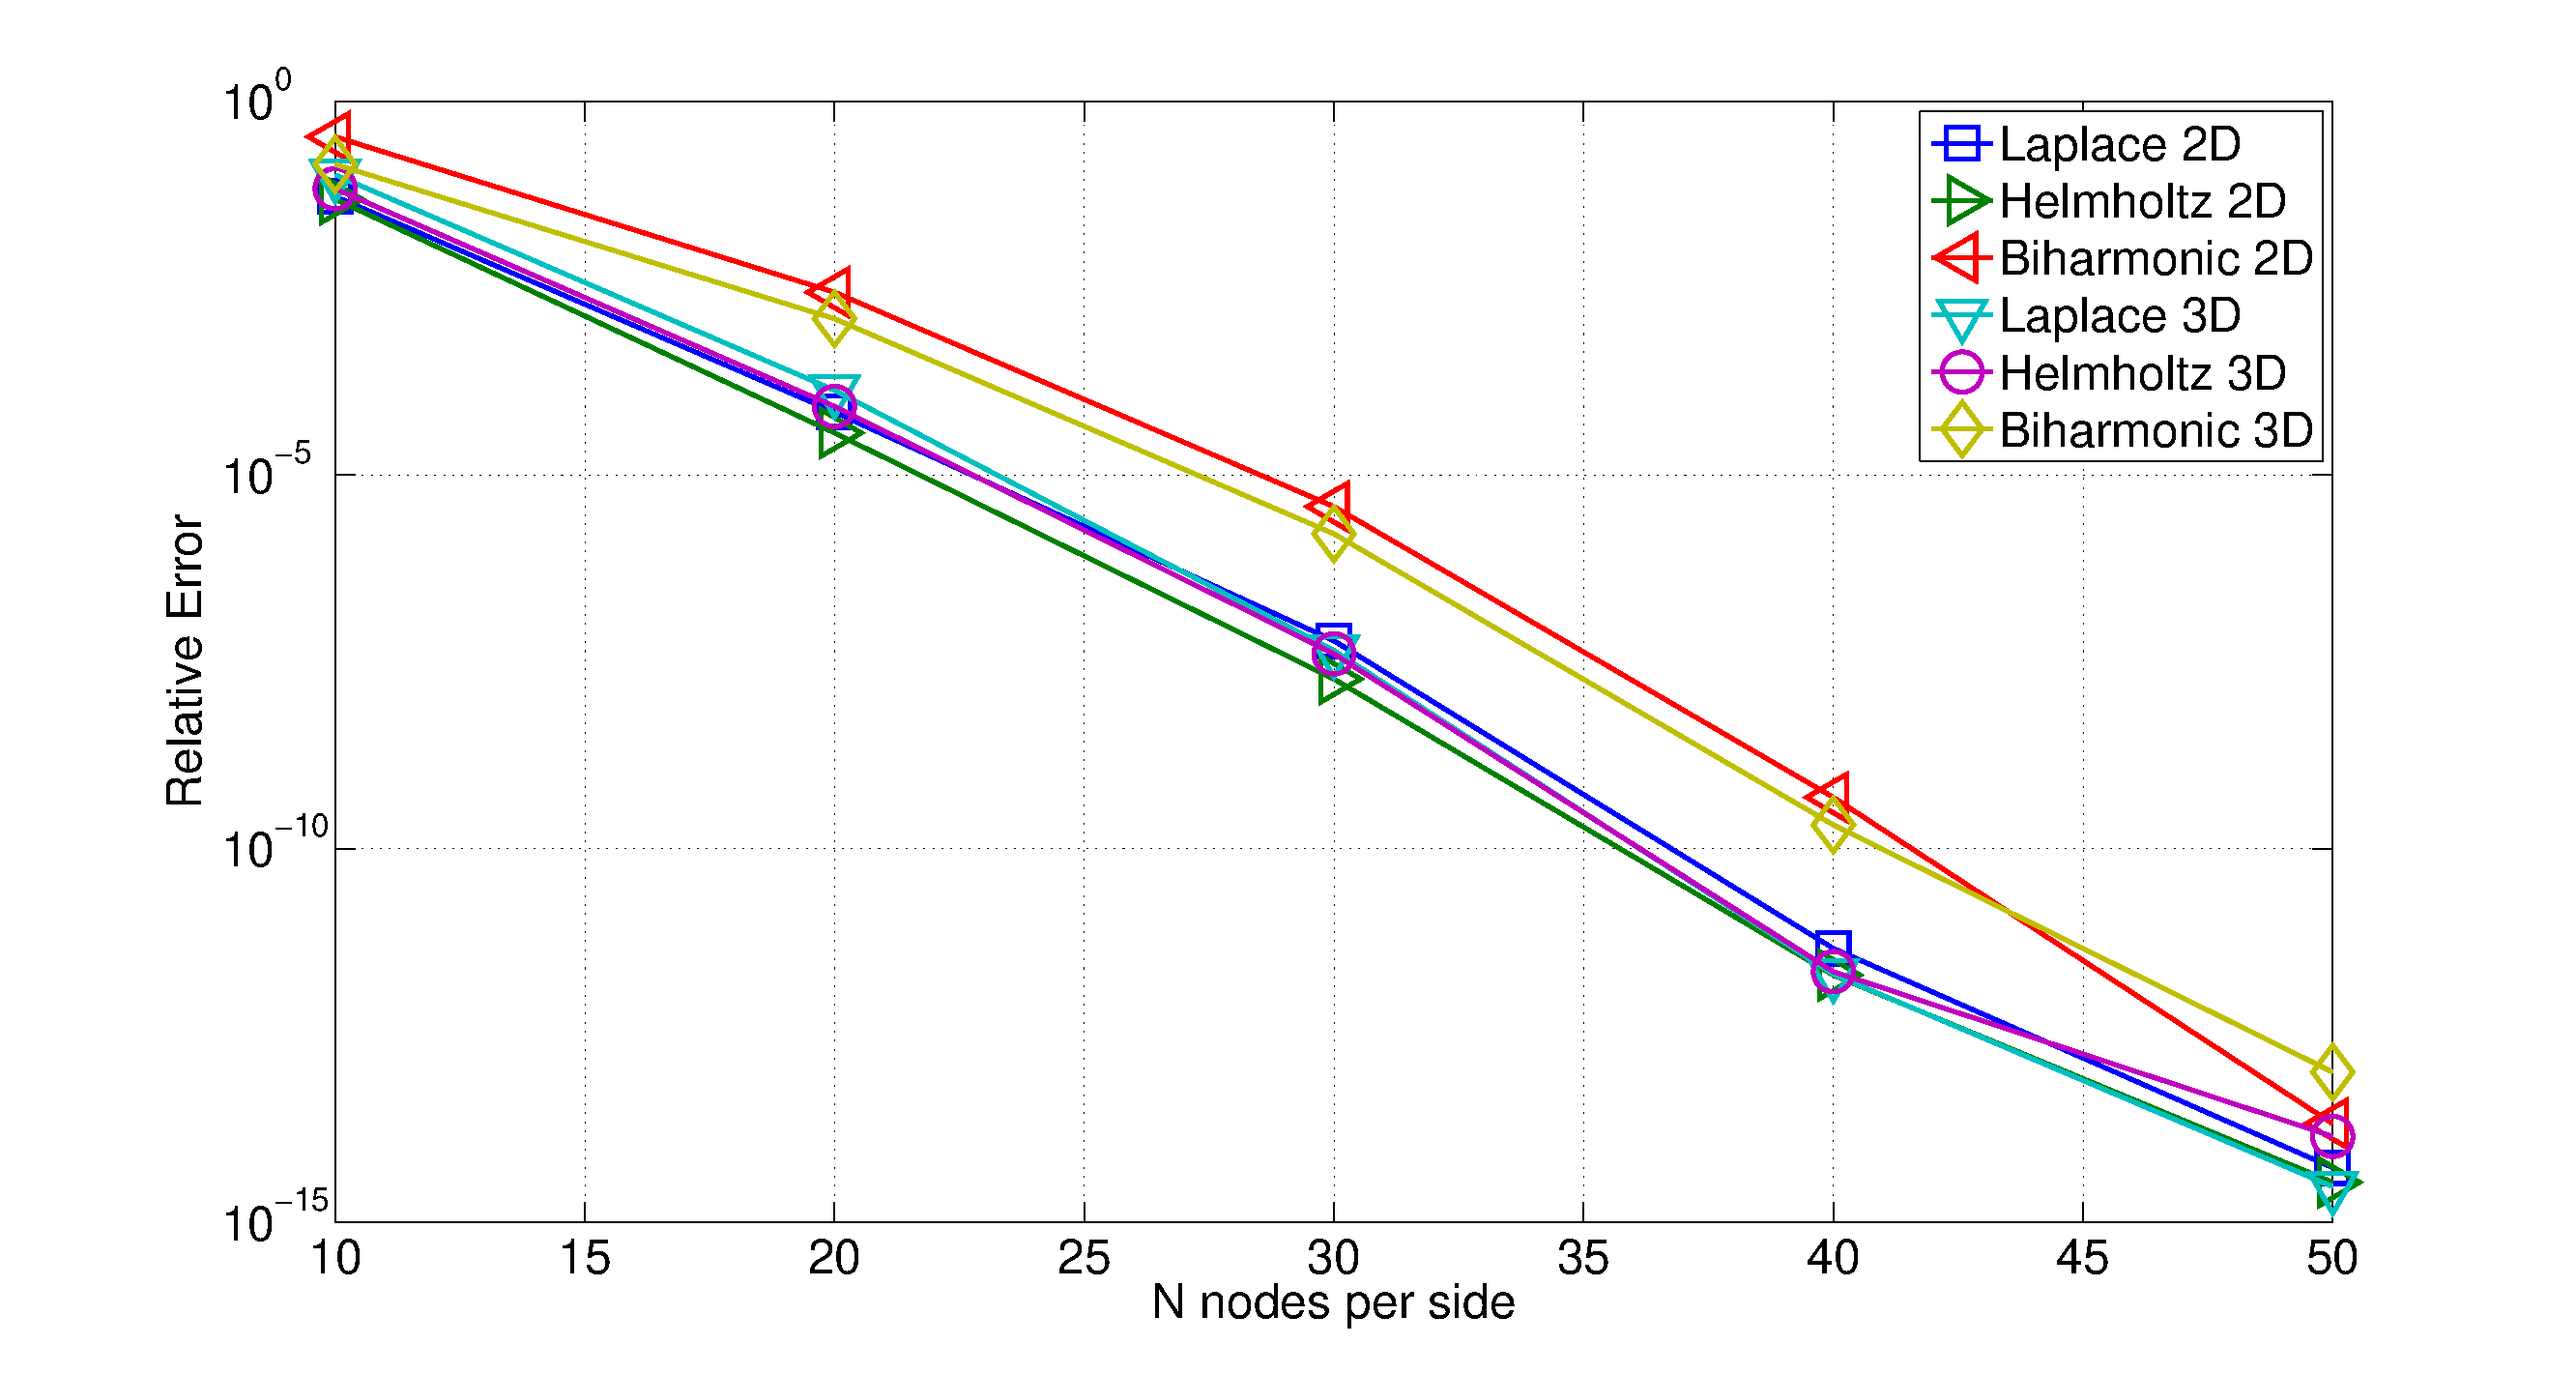
\includegraphics[height=0.72\textheight]{Error_Convolution.pdf}

\vspace{1mm}
\scriptsize Smooth Gaussian data show rapid convergence for Poisson, Helmholtz, and biharmonic kernels in 2D and 3D.
\end{frame}

%================================================================
\begin{frame}{Variable-coefficient elliptic equations}
\small
Consider
\[
  \nabla\cdot \epsilon(\x)\nabla \phi-\lambda^2\phi=\rho(\x).
\]
When $\epsilon$ is a smooth perturbation of a constant background, the PDE can be rewritten as a volume integral equation.

\vspace{2mm}
The TKM provides fast, high-order application of the volume potential inside each matrix-vector product.
\end{frame}

%================================================================
\begin{frame}{Poisson-Boltzmann example}
\centering
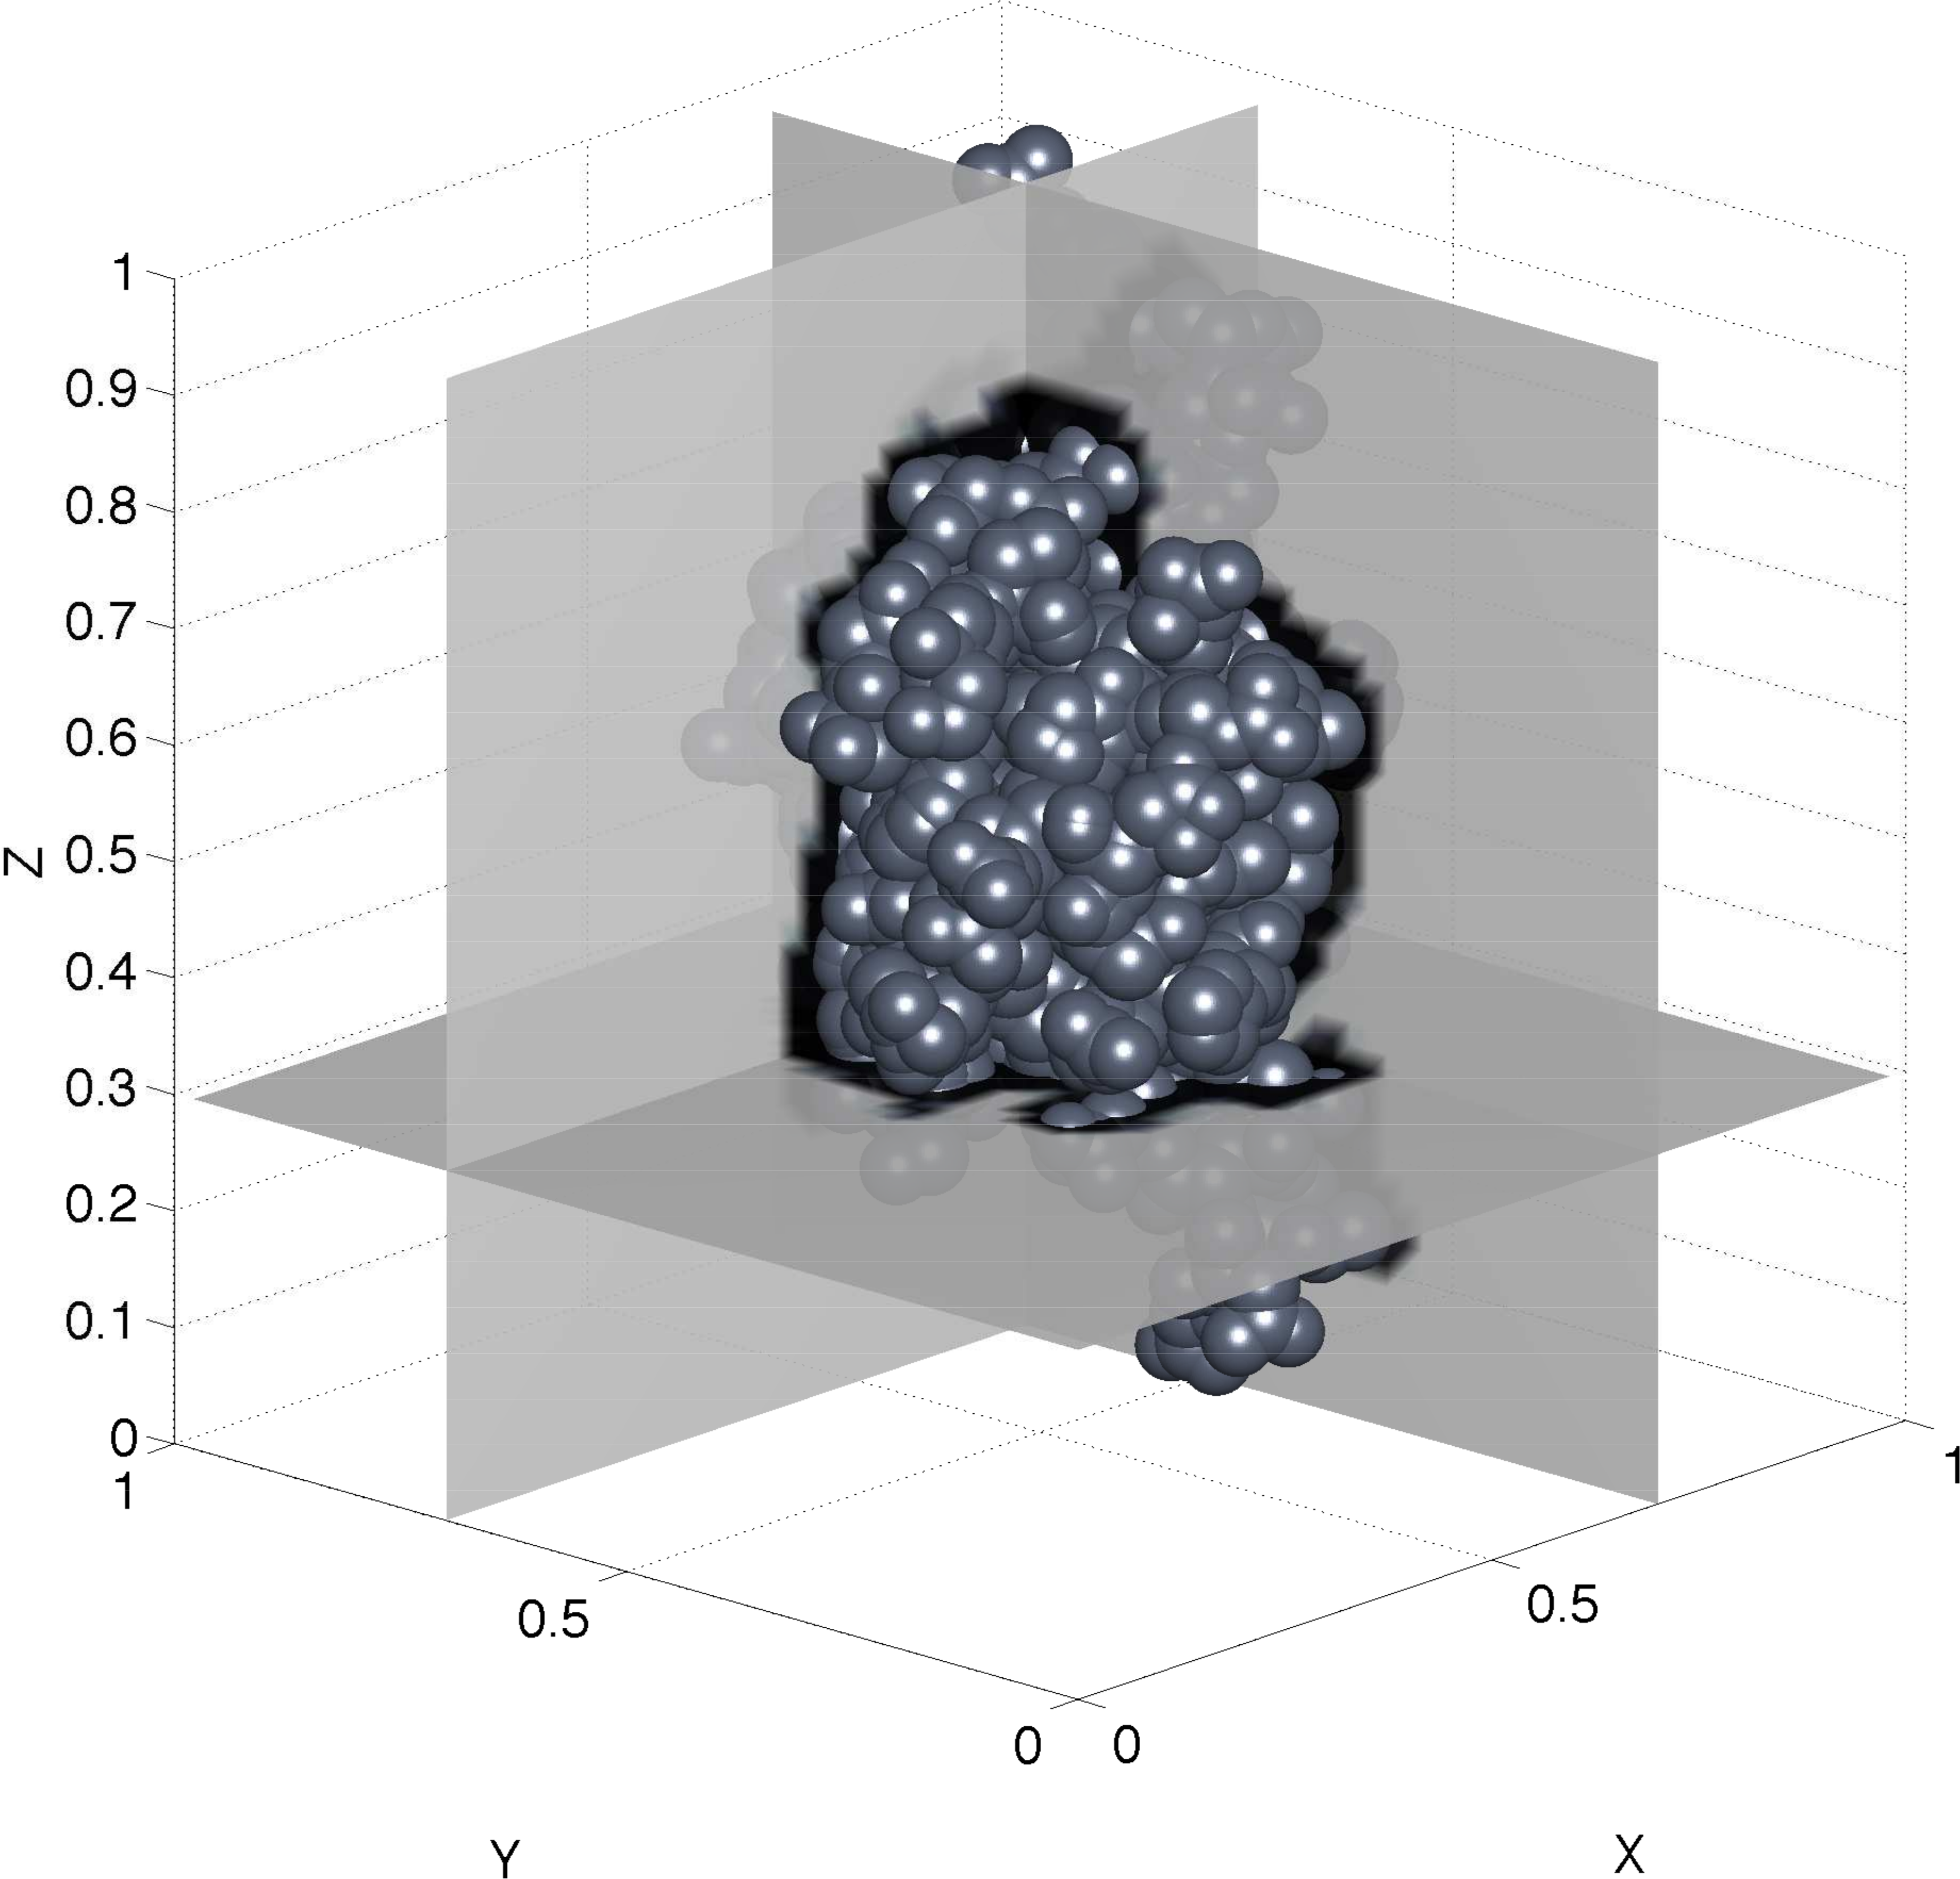
\includegraphics[height=0.78\textheight]{Protein_3D_paper_cropped.png}

\vspace{1mm}
\scriptsize Smooth dielectric functions in molecular electrostatics lead to large 3D volume integral equations.
\end{frame}

%================================================================
\begin{frame}{Variable-coefficient Poisson volume integral equation}
\small
Restricting to the Poisson case, write
\[
  \phi(\x)=\Vop_0[\sigma](\x),
  \qquad
  \Vop_0[\sigma](\x)=
  \int_{\R^3}\frac{1}{4\pi|\x-\y|}
  \sigma(\y)\dd V_{\y}.
\]
Then one obtains a second-kind equation of the form
\[
  -\epsilon(\x)\sigma(\x)
  +
  \nabla\epsilon(\x)\cdot
  \nabla\Vop_0[\sigma](\x)
  =
  \rho(\x).
\]

\vspace{1mm}
Each GMRES matvec uses TKM for the Newtonian potential and its gradient.
\end{frame}

%================================================================
\begin{frame}{Variable-coefficient matvec structure}
\small
The previous equation has the schematic form
\[
  A\sigma
  =
  -\epsilon\sigma+\nabla\epsilon\cdot\nabla \Vop_0[\sigma],
  \qquad
  \Vop_0[\sigma](\x)=
  \int_{\R^3}\frac{\sigma(\y)}{4\pi|\x-\y|}\dd V_{\y}.
\]
One Krylov matvec is:
\begin{enumerate}
  \item compute $v=\Vop_0[\sigma]$ by TKM;
  \item compute $\nabla v$ by spectral differentiation or derivative stencils;
  \item multiply pointwise by $\nabla\epsilon$;
  \item add the diagonal term $-\epsilon\sigma$.
\end{enumerate}

\vspace{1mm}
The computational bottleneck is a translation-invariant convolution; all
coefficient dependence is pointwise.
\end{frame}

%================================================================
\begin{frame}{Lippmann-Schwinger scattering}
\small
Let $\phi=\phi^{\rm inc}+\phi^{\rm scat}$, with $q$ supported in $D$ and
\[
  (\Delta+k^2)\phi^{\rm inc}=0.
\]
Then the scattered field satisfies
\[
  \Delta\phi^{\rm scat}+k^2(1+q(\x))\phi^{\rm scat}
  =
  -k^2q(\x)\phi^{\rm inc}.
\]
Its outgoing Green's-function representation is
\[
  \phi^{\rm scat}(\x)
  =
  k^2\int_D G_k(\x-\y)q(\y)\phi(\y)\dd\y
  =
  \int_D G_k(\x-\y)\sigma(\y)\dd\y,
\]
where $\sigma=k^2q(\phi^{\rm inc}+\phi^{\rm scat})$.  Substitution gives
\[
  -\sigma+k^2q(\x)\int_D G_k(\x-\y)\sigma(\y)\dd\y
  =
  -k^2q(\x)\phi^{\rm inc}.
\]

\vspace{2mm}
The TKM supplies the fast Helmholtz volume potential.
\end{frame}

%================================================================
\begin{frame}{Large scattering example}
\centering
\includegraphics[height=0.78\textheight]{SCFB_L80_v3_cropped.png}

\vspace{1mm}
\scriptsize Scattering from a smoothly filtered disk, with a domain size measured in wavelengths.
\end{frame}

%================================================================
\begin{frame}{Complexity}
\small
On an $N^d$ grid, one potential evaluation uses one forward FFT and one
inverse FFT:
\[
  \text{cost}=\cO(N^d\log N).
\]

\begin{itemize}
  \item A precomputed stencil amortizes the direct spectral construction.
  \item Each requested derivative requires one additional inverse FFT.
  \item Memory scales with the padded tensor grid.
\end{itemize}
\end{frame}

%================================================================
\begin{frame}{Choosing $L$ in practice}
\small
\begin{itemize}
  \item $L$ must exceed the maximum source-target distance in the required region.
  \item Larger $L$ increases oscillations in $\widehat{G^L}$.
  \item Smaller $L$ truncates real interactions and gives a biased answer.
\end{itemize}

\vspace{2mm}
The geometry determines the smallest admissible $L$; its value then determines
how finely the oscillatory multiplier must be resolved.
\end{frame}

%================================================================
\begin{frame}{Board derivation: truncated kernel multiplier}
\small
The derivation worth doing live is:
\[
  G_0^L(r)=\frac{1}{4\pi r}\chi_{[0,L]}(r)
\]
\[
  \widehat{G_0^L}(s)
  =
  4\pi\int_0^L
  \frac{\sin(sr)}{sr}\frac{1}{4\pi r}r^2\dd r
  =
  \frac{1-\cos(Ls)}{s^2}.
\]
Then point out:
\[
  \frac{1-\cos(Ls)}{s^2}
  =
  2\left(\frac{\sin(Ls/2)}{s}\right)^2
\]
is smooth at $s=0$.
\end{frame}

%================================================================
\begin{frame}{Exercise: TKM apply step}
\small
Implement 3D Poisson TKM:
\begin{enumerate}
  \item sample a Gaussian density on a uniform grid;
  \item zero-pad;
  \item multiply by $\widehat{G_0^L}(\s)$;
  \item inverse FFT;
  \item compare against the analytic error-function solution.
\end{enumerate}

\vspace{2mm}
Then repeat with a derivative by multiplying by $\ii s_\ell$.
\end{frame}

%================================================================
\begin{frame}{Frequency grid bookkeeping}
\small
On a box of side length $P$, FFT frequencies are
\[
  s_\ell=\frac{2\pi m_\ell}{P},
  \qquad
  m_\ell=-\frac{M}{2},\ldots,\frac{M}{2}-1.
\]

\begin{itemize}
  \item Evaluate $\widehat{G^L}(|\s|)$ at these tensor-product frequencies.
  \item Use the same normalization convention throughout.
  \item Treat the zero frequency and removable singular frequencies by limits.
\end{itemize}
\end{frame}

%================================================================
\begin{frame}{Removable singularities in code}
\small
Raw formulas such as
\[
  2\left(\frac{\sin(Ls/2)}{s}\right)^2
\]
should not be evaluated naively for very small $s$.

\vspace{2mm}
Use a local expansion:
\[
  \widehat{G_0^L}(s)=
  \frac{L^2}{2}
  -\frac{L^4s^2}{24}
  +\frac{L^6s^4}{720}
  +\cO(s^6).
\]

\vspace{1mm}
The same principle applies at $s=k$ for Helmholtz.
\end{frame}

%================================================================
\begin{frame}{Precompute/apply workflow}
\small
\begin{center}
\begin{tikzpicture}[>=Latex,node distance=7mm]
  \node[draw,rounded corners=2pt,fill=black!4,inner sep=5pt] (delta) {delta source};
  \node[draw,rounded corners=2pt,fill=black!4,inner sep=5pt,right=of delta] (fft4) {$4N$ TKM solve};
  \node[draw,rounded corners=2pt,fill=black!4,inner sep=5pt,right=of fft4] (stencil) {stencil $T$};
  \node[draw,rounded corners=2pt,fill=black!4,inner sep=5pt,below=of stencil] (apply) {$2N$ convolution};
  \node[draw,rounded corners=2pt,fill=black!4,inner sep=5pt,left=of apply] (rhs) {new source};
  \draw[->,thick,CCMorange] (delta) -- (fft4);
  \draw[->,thick,CCMorange] (fft4) -- (stencil);
  \draw[->,thick,CCMorange] (rhs) -- (apply);
  \draw[->,thick,CCMorange] (stencil) -- (apply);
\end{tikzpicture}
\end{center}

\vspace{2mm}
The expensive construction is amortized over many right-hand sides or many matvecs.
\end{frame}

%================================================================
\begin{frame}{Conditions for TKM}
\small
TKM assumes:
\begin{itemize}
  \item a uniform tensor grid covering all source and target points;
  \item a truncation radius $L$ that covers the required source-target distances;
  \item sufficient padding to resolve the oscillatory truncated multiplier;
  \item smooth, sufficiently resolved source data for high-order Fourier convergence;
  \item memory for the padded tensor grid.
\end{itemize}
\end{frame}

%================================================================
\begin{frame}{TKM implementation requirements}
\small
\begin{enumerate}
  \item Decide the source box and target box.
  \item Choose $L$ larger than the maximum interaction distance.
  \item Choose padding and frequency grid sizes.
  \item Evaluate $\widehat{G^L}$ with series handling at removable singularities.
  \item Validate on Gaussian sources with analytic solutions.
  \item Precompute the stencil if many applications are needed.
\end{enumerate}
\end{frame}

%================================================================
\begin{frame}{TKM summary}
\small
\begin{enumerate}
  \item Free-space convolution is long range and singular.
  \item Truncating the kernel in physical space is exact if $L$ exceeds all relevant distances.
  \item The truncated spectral multiplier is smooth.
  \item For smooth volume data, the trapezoidal rule plus standard FFT gives
  high-order volume potentials.
  \item A precomputed stencil gives a high-order Nystr\"om matrix interpretation.
\end{enumerate}
\end{frame}

%================================================================
\begin{frame}{Break}
\centering
\vspace{18mm}
{\Large 10 minute break}

\vspace{8mm}
After the break: function extension from complex domains to an enclosing box.
\end{frame}

%================================================================
\section{Function Extension}

\begin{frame}{Function extension objectives}
\small
The main mathematical and algorithmic objectives are:
\begin{enumerate}
  \item explain why data on a complex domain must be extended smoothly to an enclosing box;
  \item derive the finite derivative-matching conditions;
  \item compute weights from Lagrange basis values;
  \item state why Chebyshev nodes are optimal for this extension norm;
  \item describe the windowed extension used in PDE solvers;
  \item outline a particular-solution plus boundary-integral correction on a complex domain.
\end{enumerate}
\end{frame}

%================================================================
\begin{frame}{Function extension from a complex domain}
\small
For PDE data specified only on a complex domain, choose an enclosing
rectangular box for the FFT grid:
\[
  \mathcal{L}u(\x)=f(\x),\qquad \x\in\Omega.
\]

\vspace{2mm}
To compute a particular solution by FFT, construct a smooth function $f^e$ on
the box:
\[
  f^e|_\Omega=f,
  \qquad
  f^e\text{ smoothly rolls off outside }\Omega.
\]
\end{frame}

%================================================================
\begin{frame}{Loss of smoothness under zero extension}
\small
The trivial extension
\[
  f^e(\x)=
  \begin{cases}
  f(\x),& \x\in\Omega,\\
  0,& \x\notin\Omega
  \end{cases}
\]
is generally discontinuous across $\partial\Omega$. Even when $f$ vanishes on
the boundary, its normal derivatives generally do not match.

\begin{itemize}
  \item Fourier coefficients decay slowly.
  \item Gibbs oscillations contaminate the particular solution.
  \item The boundary correction must remove a rough error.
\end{itemize}
\end{frame}

%================================================================
\begin{frame}{Extension objective}
\small
Let $B\supset\overline{\Omega}$ be an enclosing box. Given
$f\in C^n(\overline{\Omega})$, construct
\[
  E_n[f]\in C^n(B)
\]
such that
\[
  E_n[f](\x)=f(\x),\qquad \x\in\Omega,
\]
and such that its exterior continuation is confined to a tubular neighborhood
of $\partial\Omega$ and smoothly windowed to zero.

\begin{block}{Design constraint}
The extension should be local, explicit, and lower cost than the FFT solve.
\end{block}
\end{frame}

%================================================================
\begin{frame}{Seeley's extension on the half-line}
\small
Let $f\in C^\infty([0,\infty))$. For $x<0$, the points $-t_jx$ lie in the
original half-line when $t_j\ge 0$. Choose:
\begin{itemize}
  \item dilation parameters $0\le t_j\uparrow\infty$ and weights $w_j$ with
  $\sum_j|w_j|t_j^m<\infty$ for every $m\ge0$;
  \item a smooth cutoff $\chi\in C_c^\infty([0,\infty))$ with
  $\chi=1$ near $0$.
\end{itemize}
Seeley's extension has the form
\[
  E_\infty[f](x)
  =
  \sum_{j=0}^{\infty}w_j f(-t_jx)\chi(-t_jx),
  \qquad x<0.
\]
For $x\ge0$, set $E_\infty[f](x)=f(x)$.

\vfill
\scriptsize R. T. Seeley, \emph{Extension of $C^\infty$ functions defined in a half space},
\emph{Proceedings of the American Mathematical Society}, 15 (1964), 625--626.
\end{frame}

%================================================================
\begin{frame}{Derivative matching gives the moment conditions}
\small
Since $\chi$ is constant near $0$, it contributes no derivatives at the
boundary. For $i\ge0$,
\[
  E_\infty^{(i)}[f](0^-)
  =
  \sum_{j=0}^{\infty}w_j(-t_j)^i f^{(i)}(0^+)
  =
  f^{(i)}(0^+)\sum_{j=0}^{\infty}w_j(-t_j)^i.
\]
To obtain a smooth extension, the left and right derivatives must agree:
\[
  E_\infty^{(i)}[f](0^-)=f^{(i)}(0^+).
\]
Since this must hold for every $f$, the weights must satisfy
\[
  \sum_{j=0}^{\infty}w_j(-t_j)^i=1
  \qquad\Longleftrightarrow\qquad
  \sum_{j=0}^{\infty}w_jt_j^i=(-1)^i,
  \qquad i=0,1,\ldots.
\]
\end{frame}

%================================================================
\begin{frame}{Finite $C^n$ extension formula}
\small
For a $C^n$ extension, retain $n+1$ terms with distinct
$0\le t_0<\cdots<t_n$. For $x<0$, define
\[
  E_n[f](x)=
  \sum_{j=0}^n w_j f(-t_jx).
\]
The finite weights enforce the first $n+1$ moment conditions:
\[
  \sum_{j=0}^n w_jt_j^i=(-1)^i,
  \qquad i=0,\ldots,n.
\]
\end{frame}

%================================================================
\begin{frame}{The finite Vandermonde system}
\small
The weights satisfy
\[
\begin{bmatrix}
1&1&\cdots&1\\
t_0&t_1&\cdots&t_n\\
\vdots&\vdots&&\vdots\\
t_0^n&t_1^n&\cdots&t_n^n
\end{bmatrix}
\begin{bmatrix}
w_0\\w_1\\\vdots\\w_n
\end{bmatrix}
=
\begin{bmatrix}
1\\-1\\\vdots\\(-1)^n
\end{bmatrix}.
\]

\vspace{2mm}
Solving this system numerically is a poor way to compute the weights. We derive explicit formulas.
\end{frame}

%================================================================
\begin{frame}{Normal coordinates on a smooth domain}
\small
Let $y\in\partial\Omega$ and let $\nu_y$ be the outward unit normal.
For $|r|$ small,
\[
  (y,r)\mapsto y+r\nu_y
\]
is a diffeomorphism onto a tubular neighborhood.

\vspace{2mm}
This reduces local extension to a one-dimensional normal-direction problem.
\end{frame}

%================================================================
\begin{frame}{Tubular-neighborhood restriction}
\small
The normal map
\[
  F(y,r)=y+r\nu_y
\]
is valid only inside the reach of the boundary.  In 2D, if $\kappa(y)$ is the
signed curvature for the chosen normal direction, the Jacobian contains
\[
  J(y,r)=1+\kappa(y)r
\]
for the normal coordinate $x=F(y,r)$.

\vspace{1mm}
Therefore the extension width must satisfy two geometric constraints:
\begin{itemize}
  \item normals from different boundary points should not intersect in the layer;
  \item sample points $y-t_jr\nu_y$ must remain inside $\Omega$.
\end{itemize}

\vspace{1mm}
High extension order cannot fix a normal map that is no longer one-to-one.
\end{frame}

%================================================================
\begin{frame}{Geometry of the EFJ extension}
\begin{center}
\begin{tikzpicture}[scale=1.0,>=Latex]
  \draw[very thick] plot[smooth] coordinates {(-3,-0.6) (-2,-0.1) (-0.7,0.2) (0.8,0.0) (2.9,0.45)};
  \coordinate (y) at (-0.4,0.17);
  \fill[SFdark] (y) circle (2pt) node[below=3pt,black] {$y$};
  \draw[->,thick,SFdark] (y) -- ++(0.22,0.95) node[above] {$\nu_y$};
  \fill[CCMorange] ($(y)+(0.35,1.15)$) circle (2.3pt) node[right,black] {target};
  \foreach \t in {0.25,0.55,0.85}
    \fill[black] ($(y)-\t*(0.35,1.15)$) circle (1.6pt);
  \node[align=center] at (1.2,-1.0) {\scriptsize exterior target samples\\[-1pt]\scriptsize interior points on same normal};
\end{tikzpicture}
\end{center}
\end{frame}

%================================================================
\begin{frame}{Extension formula on a domain}
\small
For an exterior point written as
\[
  \x=y+r\nu_y,\qquad r>0,
\]
define
\[
  E_n[f](y+r\nu_y)
  =
  \sum_{j=0}^n w_j f(y-t_jr\nu_y).
\]

\begin{itemize}
  \item The sample points lie inside $\Omega$.
  \item The sample locations depend on the exterior distance $r$.
  \item Tangential smoothness is inherited from $f$ and the boundary.
\end{itemize}
\end{frame}

%================================================================
\begin{frame}{Tangential smoothness of the EFJ extension}
\small
The formula samples along a normal line:
\[
  y+r\nu_y
  \mapsto
  y-t_jr\nu_y.
\]
If $y$ varies smoothly along $\partial\Omega$, then the sample points vary smoothly along the boundary.

\vspace{2mm}
Thus only normal derivatives need to be matched explicitly. Tangential regularity follows from smooth geometry and smooth $f$.
\end{frame}

%================================================================
\begin{frame}{Moment conditions as polynomial extrapolation}
\small
Let $\mathbb{P}_n$ denote the polynomials of degree at most $n$.
For
\[
  q(x)=\sum_{k=0}^n a_kx^k\in\mathbb{P}_n,
\]
the moment conditions give
\[
  \begin{aligned}
    \sum_{i=0}^n w_iq(t_i)
    &=
    \sum_{k=0}^n a_k\left(\sum_{i=0}^n w_it_i^k\right) \\
    &=
    \sum_{k=0}^n a_k(-1)^k
    =q(-1).
  \end{aligned}
\]

\begin{block}{Meaning of the moment system}
The weights extrapolate every polynomial in $\mathbb{P}_n$ from the nodes
$t_0,\ldots,t_n$ to the point $-1$.
\end{block}
\end{frame}

%================================================================
\begin{frame}{Lagrange interpolation identifies the weights}
\small
For the distinct nodes $t_0,\ldots,t_n$, let
\[
  l_i(x)=
  \prod_{m\ne i}\frac{x-t_m}{t_i-t_m}
\]
be the Lagrange basis. Every $q\in\mathbb{P}_n$ satisfies
\[
  q(x)=\sum_{i=0}^n q(t_i)l_i(x).
\]
Evaluating at $x=-1$ gives
\[
  q(-1)=\sum_{i=0}^n q(t_i)l_i(-1).
\]
Taking $q=l_k$ in the preceding slide's extrapolation identity yields
\[
  \boxed{w_k=l_k(-1),\qquad k=0,\ldots,n.}
\]

\vspace{1mm}
The distinct nodes make the Vandermonde matrix invertible, so these weights are unique.
\end{frame}

%================================================================
\begin{frame}{Explicit Lagrange weight formula}
\small
Evaluating the Lagrange basis gives
\[
  w_i=(-1)^i
  \prod_{m=0}^{i-1}\frac{1+t_m}{t_i-t_m}
  \prod_{m=i+1}^{n}\frac{1+t_m}{t_m-t_i}.
\]

\begin{itemize}
  \item The signs alternate.
  \item The formula is explicit once nodes are chosen.
  \item The remaining design choice is the node set.
\end{itemize}
\end{frame}

%================================================================
\begin{frame}{Metrics for extension quality}
\small
For nodes $0\le t_i\le a$, a function $f$ on $[0,a]$ is extended to
$[-1,0]$ with
\[
  \|E_n f\|_{L^\infty([-1,0])}
  \le
  \|w\|_1\|f\|_{L^\infty([0,a])}.
\]

\vspace{2mm}
We choose nodes by minimizing
\[
  \|w\|_1=\sum_{i=0}^n|w_i|.
\]
\end{frame}

%================================================================
\begin{frame}{The node problem is a polynomial minimization problem}
\small
For increasing nodes, the explicit formula gives
\[
  \operatorname{sgn}(w_i)=(-1)^i.
\]
Define
\[
  P(x)=\sum_{i=0}^n(-1)^i l_i(x).
\]
\[
  P(t_i)=(-1)^i,
  \qquad
  \|w\|_1
  =
  \sum_{i=0}^n(-1)^i l_i(-1)
  =
  P(-1).
\]
Thus choosing the nodes is equivalent to
\[
  \boxed{
    \begin{aligned}
      \text{minimize}\quad & P(-1),\\
      \text{subject to}\quad & P\in\mathbb{P}_n,\qquad P(t_i)=(-1)^i\quad(i=0,\ldots,n),\\
      & 0\le t_0<\cdots<t_n\le a.
    \end{aligned}
  }
\]

\vspace{1mm}
The node optimization has become an equioscillation problem for a degree-$n$ polynomial.
\end{frame}

%================================================================
\begin{frame}{A minimizer cannot overshoot}
\small
Let $p^\ast$ be a minimizer. Suppose that
$p^\ast(t^\circ)>1$ at an interior point $t^\circ$. Replace the closest node
$t_j^\ast$ at which $p^\ast(t_j^\ast)=1$ by $t^\circ$, and let $q$ interpolate
the same alternating values at the modified nodes.

\vspace{1mm}
This comparison gives $j$ even, $c>0$, and
\[
  p^\ast(x)-q(x)
  =
  c\prod_{i=0}^{j-1}(x-t_i^\ast)
   \prod_{i=j+1}^{n}(t_i^\ast-x).
\]
Consequently,
\[
  p^\ast(-1)-q(-1)
  =
  c\prod_{i=0}^{j-1}(1+t_i^\ast)
   \prod_{i=j+1}^{n}(1+t_i^\ast)>0.
\]
But $q$ is another admissible equioscillating polynomial with a smaller value at $-1$,
a contradiction. The case $p^\ast(t^\circ)<-1$ is analogous. Hence
\[
  \boxed{|p^\ast(x)|\le 1,\qquad x\in[0,a].}
\]
\end{frame}

%================================================================
\begin{frame}{Bounded equioscillation is unique}
\small
Suppose $p_1$ and $p_2$ are two bounded equioscillating degree-$n$ polynomials.
Their roots interlace their alternating nodes, so both are positive to the left of $[0,a]$.
If they differed, exchange their labels and choose $\xi<0$ such that
\[
  0<p_1(\xi)<p_2(\xi),
  \qquad
  \alpha=\frac{p_1(\xi)}{p_2(\xi)}\in(0,1).
\]
For
\[
  q(x)=p_1(x)-\alpha p_2(x),
\]
we have $q(\xi)=0$. At the alternating nodes $s_i$ of $p_1$,
\[
  \operatorname{sgn}q(s_i)=(-1)^i,
  \qquad\text{because}\qquad |\alpha p_2(s_i)|<1.
\]
Thus $q$ has $n$ roots in $(0,a)$ and one at $\xi$, impossible unless $q\equiv0$.
That would give $|p_1|=\alpha|p_2|<1$ on $[0,a]$, contradicting $|p_1(s_i)|=1$.
\end{frame}

%================================================================
\begin{frame}{Chebyshev solves the minimization problem}
\small
The scaled Chebyshev polynomial
\[
  T_n\!\left(1-\frac{2x}{a}\right)
\]
satisfies $\left|T_n(1-2x/a)\right|\le1$ on $[0,a]$. At
\[
  t_i^\ast=
  \frac{a}{2}\left(1-\cos\frac{i\pi}{n}\right),
  \qquad i=0,\ldots,n,
\]
it has the alternating values
\[
  T_n\!\left(\cos\frac{i\pi}{n}\right)
  =
  (-1)^i.
\]
The preceding two slides show that a minimizer is bounded and that such an
equioscillating polynomial is unique. Therefore
\[
  \boxed{p^\ast(x)=T_n\!\left(1-\frac{2x}{a}\right),\qquad
  \min\|w\|_1=p^\ast(-1)=T_n\!\left(1+\frac{2}{a}\right).}
\]
\end{frame}

%================================================================
\begin{frame}{Optimal nodes}
\small
The optimal nodes on $[0,a]$ are shifted and scaled Chebyshev nodes of the second kind:
\[
  t_i^\ast=
  \frac{a}{2}
  \left(1-\cos\frac{i\pi}{n}\right),
  \qquad i=0,\ldots,n.
\]

\begin{itemize}
  \item $t_0^\ast=0$.
  \item $t_n^\ast=a$.
  \item Interior nodes cluster near the endpoints.
\end{itemize}
\end{frame}

%================================================================
\begin{frame}{Extrapolation amplification}
\small
The $\ell^1$ norm of the optimal weights is
\[
  \|w^\ast\|_1=T_n(1+2/a).
\]
It grows exponentially with $n$.

\begin{itemize}
  \item For fixed $a$, higher-order extrapolation amplifies data errors.
  \item Larger $a$ reduces the growth.
  \item Our reported PDE examples use $n=8$.
\end{itemize}
\end{frame}

%================================================================
\begin{frame}{Derivative bounds}
\small
Differentiate the formula:
\[
  \partial_x^\ell E_n[f](x)
  =
  \sum_{j=0}^n(-t_j)^\ell w_j
  f^{(\ell)}(-t_jx).
\]
Therefore
\[
  |\partial_x^\ell E_n[f](x)|
  \le
  \left(\sum_{j=0}^nt_j^\ell|w_j|\right)
  \|f^{(\ell)}\|_{L^\infty}.
\]

\vspace{2mm}
The same weights that control the function also control normal derivatives.
\end{frame}

%================================================================
\begin{frame}{The parameter $a$}
\small
The nodes sample points up to distance $a r$ into the domain:
\[
  y-t_jr\nu_y,\qquad 0\le t_j\le a.
\]

\begin{itemize}
  \item Larger $a$ improves conditioning.
  \item Larger $a$ requires deeper access to interior values.
  \item Geometry may limit $a$ before normals intersect or caustics appear.
\end{itemize}
\end{frame}

%================================================================
\begin{frame}{Need for a window}
\small
To place the extended data on a finite computational box, localize the
continuation with a smooth rolloff. Let $0<r_0<r_1$ be the inner and outer
extension distances, and let $c>0$ be the PSWF parameter:
\[
  E_n[f](x)=
  \left(\sum_{i=0}^nw_if(-t_ix)\right)\Phi^c(-x,r_0,r_1).
\]

\begin{itemize}
  \item $\Phi^c(s,r_0,r_1)=1$ for $s\le r_0$.
  \item $\Phi^c(s,r_0,r_1)=0$ for $s\ge r_1$.
  \item The roll-off must not introduce excessive high frequencies.
\end{itemize}
\end{frame}

%================================================================
\begin{frame}{PSWF window}
\small
We use a prolate spheroidal wave function window.
For $c>0$, define the finite Fourier transform of $h\in L^2([-1,1])$ by
\[
  F_c[h](x)=\int_{-1}^1h(t)e^{\ii cxt}\dd t.
\]
The first PSWF $\psi_0^c$ is the eigenfunction of $F_c$ associated with the
eigenvalue of largest magnitude.

\vspace{2mm}
The window based on $\psi_0^c$ limits the additional frequency content of the
extension; it is the $L^2$-optimal concentration eigenfunction.
\end{frame}

%================================================================
\begin{frame}{Window formula}
\small
Define
\[
  \Psi_0^c(x)=
  \begin{cases}
  0,&x\le -1,\\
  C_0^{-1}\int_{-1}^x\psi_0^c(t)\dd t,&x\in[-1,1],\\
  1,&x\ge 1,
  \end{cases}
\]
where
\[
  C_0=\int_{-1}^1\psi_0^c(t)\dd t.
\]
Then
\[
  \Phi^c(x,r_0,r_1)=
  1-\Psi_0^c\left(\frac{2x-(r_0+r_1)}{r_1-r_0}\right).
\]
\end{frame}

%================================================================
\begin{frame}{Illustrative 1D extension}
\centering
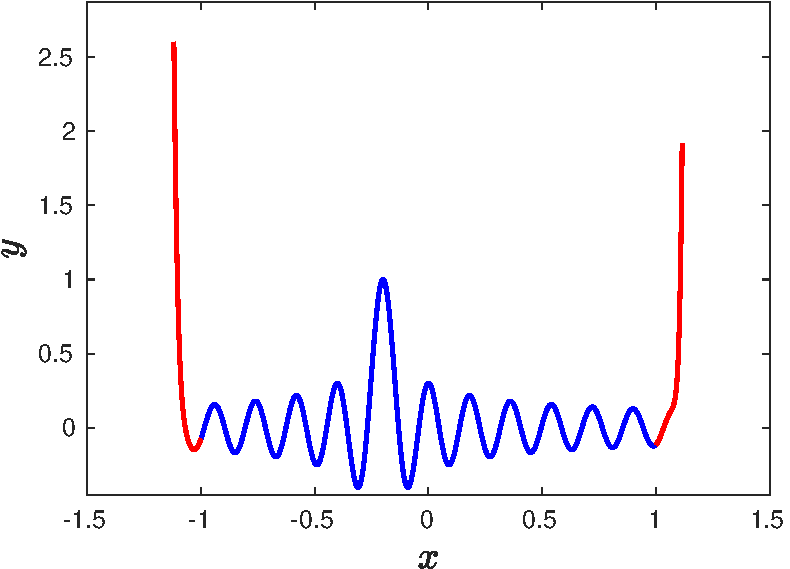
\includegraphics[height=0.72\textheight]{fig1a.pdf}

\vspace{1mm}
\scriptsize EFJ extension formula applied to an oscillatory one-dimensional test function.
\end{frame}

%================================================================
\begin{frame}{1D convergence behavior}
\centering
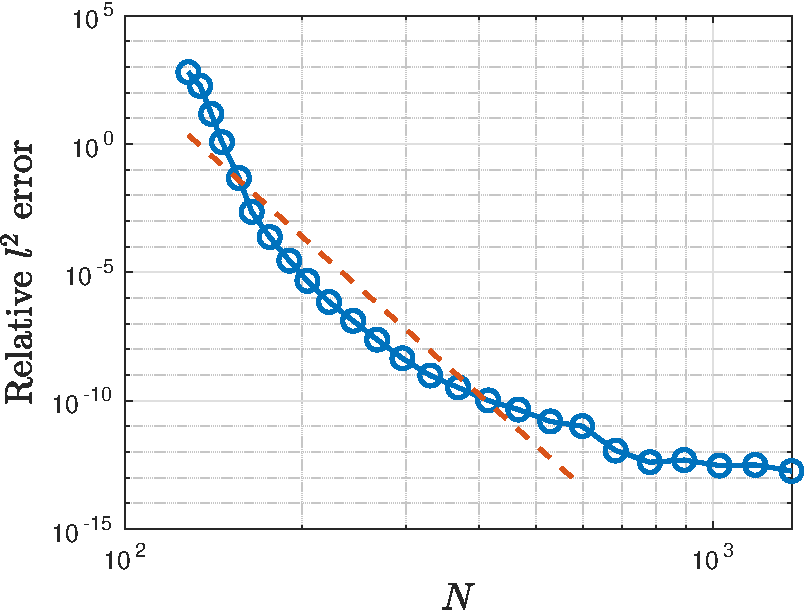
\includegraphics[height=0.72\textheight]{convergenceorder1.pdf}

\vspace{1mm}
\scriptsize The extension error decreases at the expected high order before saturating.
\end{frame}

%================================================================
\begin{frame}{Poisson BVP solver structure}
\small
Solve
\[
  -\Delta u(\x)=f(\x),\qquad \x\in\Omega,
  \qquad
  u(\x)=g(\x),\qquad \x\in\partial\Omega.
\]
Write
\[
  u=u^p+u^c.
\]

\begin{itemize}
  \item $u^p$ is a free-space particular solution computed from $f^e$ on the box.
  \item $u^c$ solves the homogeneous PDE with corrected boundary data.
  \item $u^c$ is computed by a boundary integral equation.
\end{itemize}
\end{frame}

%================================================================
\begin{frame}{Step I: bounding box and grid}
\small
Choose a rectangular box $B\supset\overline{\Omega}$ that also contains the
extension layer, and place a uniform tensor grid on $B$.

\vspace{2mm}
The grid spacing must resolve the source, the extension window, and the
boundary discretization used for the correction.
\end{frame}

%================================================================
\begin{frame}{Step II: classify grid points}
\small
Separate grid points into
\[
  \{x_i^{\rm int}\}\subset\Omega,
  \qquad
  \{x_i^{\rm ext}\}\subset\R^d\setminus\Omega.
\]

\begin{itemize}
  \item Use a point-in-domain test to label interior and exterior nodes.
  \item For exterior nodes in the extension layer, compute a boundary footpoint.
  \item Nodes farther from the boundary receive zero extended data.
\end{itemize}
\end{frame}

%================================================================
\begin{frame}{Step III: extend the source}
\small
For exterior grid points near the boundary:
\begin{enumerate}
  \item find a nearby boundary patch;
  \item find the footpoint $y$ whose normal passes through the target;
  \item evaluate interior sample points $y-t_jr\nu_y$;
  \item apply the weighted sum and window.
\end{enumerate}

\vspace{2mm}
Far exterior points are set to zero.
\end{frame}

%================================================================
\begin{frame}{Closest point and Newton iteration}
\small
For an exterior grid point $\x$, first find a closest boundary node.
Let $\gamma(s)$ parametrize the corresponding boundary patch. Then solve for
the parameter $s$ such that
\[
  \x=\gamma(s)+r\nu_{\gamma(s)}
\]
for some normal distance $r$.

\vspace{2mm}
Use this nearby point as the initial guess for a local footpoint solve.
\end{frame}

%================================================================
\begin{frame}{Step IV: FFT particular solution}
\small
For the Poisson convention $-\Delta u=f$, the particular solution is the
free-space volume potential
\[
  u^p(\x)=\int_B G_0(\x-\y)f^e(\y)\dd\y.
\]
TKM evaluates this convolution on the box using the truncated multiplier,
not the singular periodic multiplier $|\s|^{-2}$.
\end{frame}

%================================================================
\begin{frame}{Step V: boundary correction}
\small
The particular solution will not satisfy the boundary condition.
Define
\[
  g^c=g-u^p|_{\partial\Omega}.
\]
Then solve
\[
  -\Delta u^c(\x)=0,\qquad \x\in\Omega,
  \qquad
  u^c(\x)=g^c(\x),\qquad \x\in\partial\Omega.
\]

\vspace{2mm}
This is where boundary integral methods re-enter.
\end{frame}

%================================================================
\begin{frame}{Step VI: boundary integral correction}
\small
For a simply connected interior Dirichlet problem, use the double-layer
potential
\[
  \Dop[\mu](\x)
  =
  \int_{\partial\Omega}
  \partial_{\nu_{\y}}G_0(\x-\y)\mu(\y)\dd S_{\y},
  \qquad
  u^c=\Dop[\mu].
\]
The interior trace of $\Dop$ gives a second-kind boundary integral equation
for the density $\mu$.

\begin{itemize}
  \item Use a high-order quadrature for singular and close evaluation.
  \item Use GMRES and the fast multipole method (FMM) for the solve.
\end{itemize}
\end{frame}

%================================================================
\begin{frame}{Step VII: evaluate the correction}
\small
After solving for $\mu$, evaluate $u^c$ on the tensor grid:
\[
  u^c(x_i^{\rm vol})
  =
  \Dop[\mu](x_i^{\rm vol}).
\]

\begin{itemize}
  \item Use the FMM for the far field.
  \item Use close-evaluation quadrature near the boundary.
  \item Add $u=u^p+u^c$ on interior grid points.
\end{itemize}
\end{frame}

%================================================================
\begin{frame}{Overall complexity}
\small
For fixed Krylov iteration counts, we obtain the cost
\[
  \cO(N_b+M^d\log M),
\]
where:
\begin{itemize}
  \item $N_b$ is the number of boundary discretization points;
  \item $M^d$ is the number of tensor-grid points;
  \item extension and sorting are local;
  \item FFT dominates at large grid sizes.
\end{itemize}
\end{frame}

%================================================================
\begin{frame}{Example: source and extension in 2D}
\centering
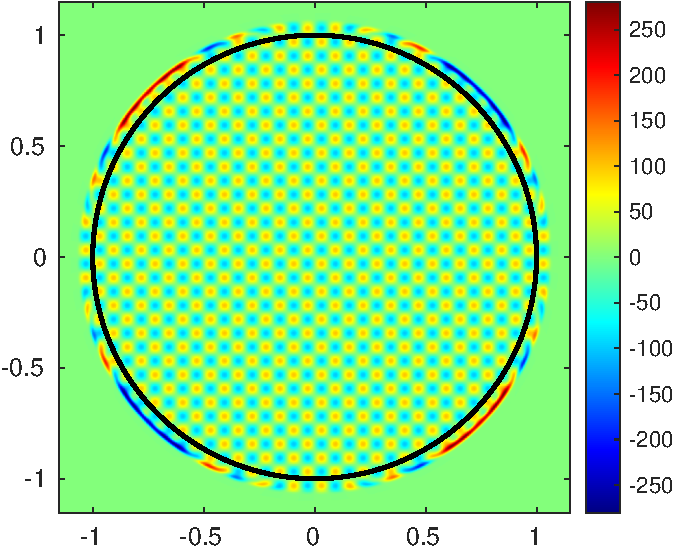
\includegraphics[height=0.72\textheight]{example1a.pdf}

\vspace{1mm}
\scriptsize Boundary, right-hand side, and eighth-order EFJ extension.
\end{frame}

%================================================================
\begin{frame}{Example: 2D convergence and timings}
\centering
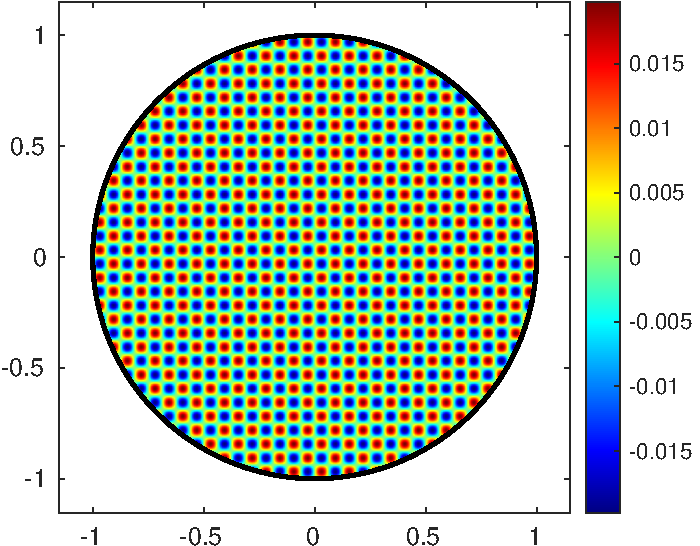
\includegraphics[height=0.72\textheight]{example1b.pdf}

\vspace{1mm}
\scriptsize The FFT step dominates asymptotically; extension remains a small fraction of the runtime.
\end{frame}

%================================================================
\begin{frame}{Example: solution and error}
\centering
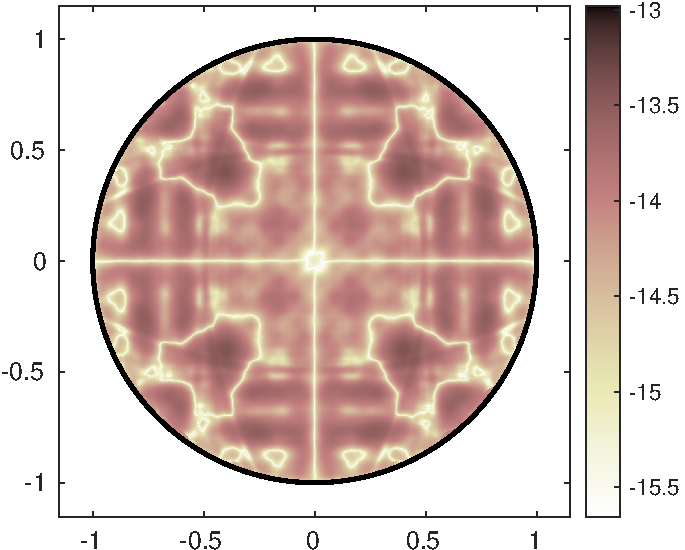
\includegraphics[height=0.72\textheight]{example1c.pdf}

\vspace{1mm}
\scriptsize High accuracy is obtained on a complex smooth domain.
\end{frame}

%================================================================
\begin{frame}{Effect of extension order}
\centering
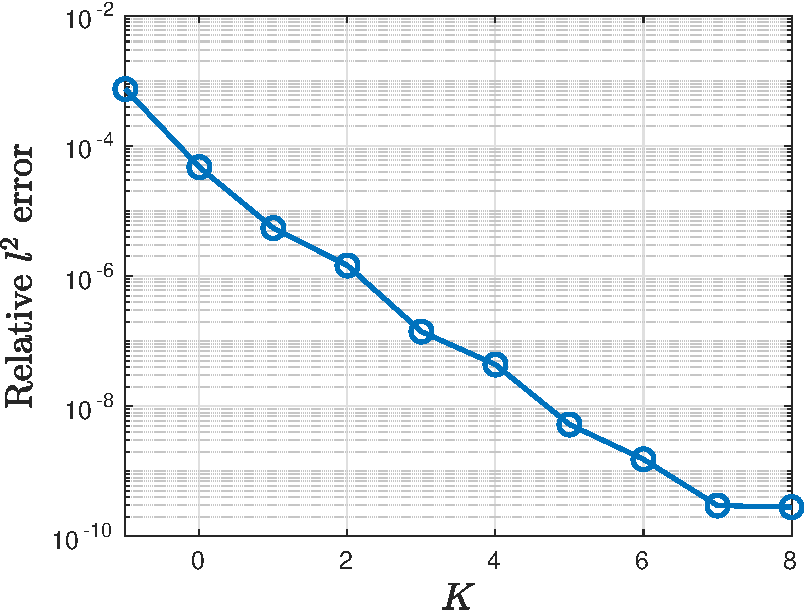
\includegraphics[height=0.72\textheight]{extensionorder1.pdf}

\vspace{1mm}
\scriptsize Increasing extension order improves the PDE solution until other errors dominate.
\end{frame}

%================================================================
\begin{frame}{3D stellarator example}
\begin{columns}[T,totalwidth=\textwidth]
\begin{column}{0.49\textwidth}
\centering
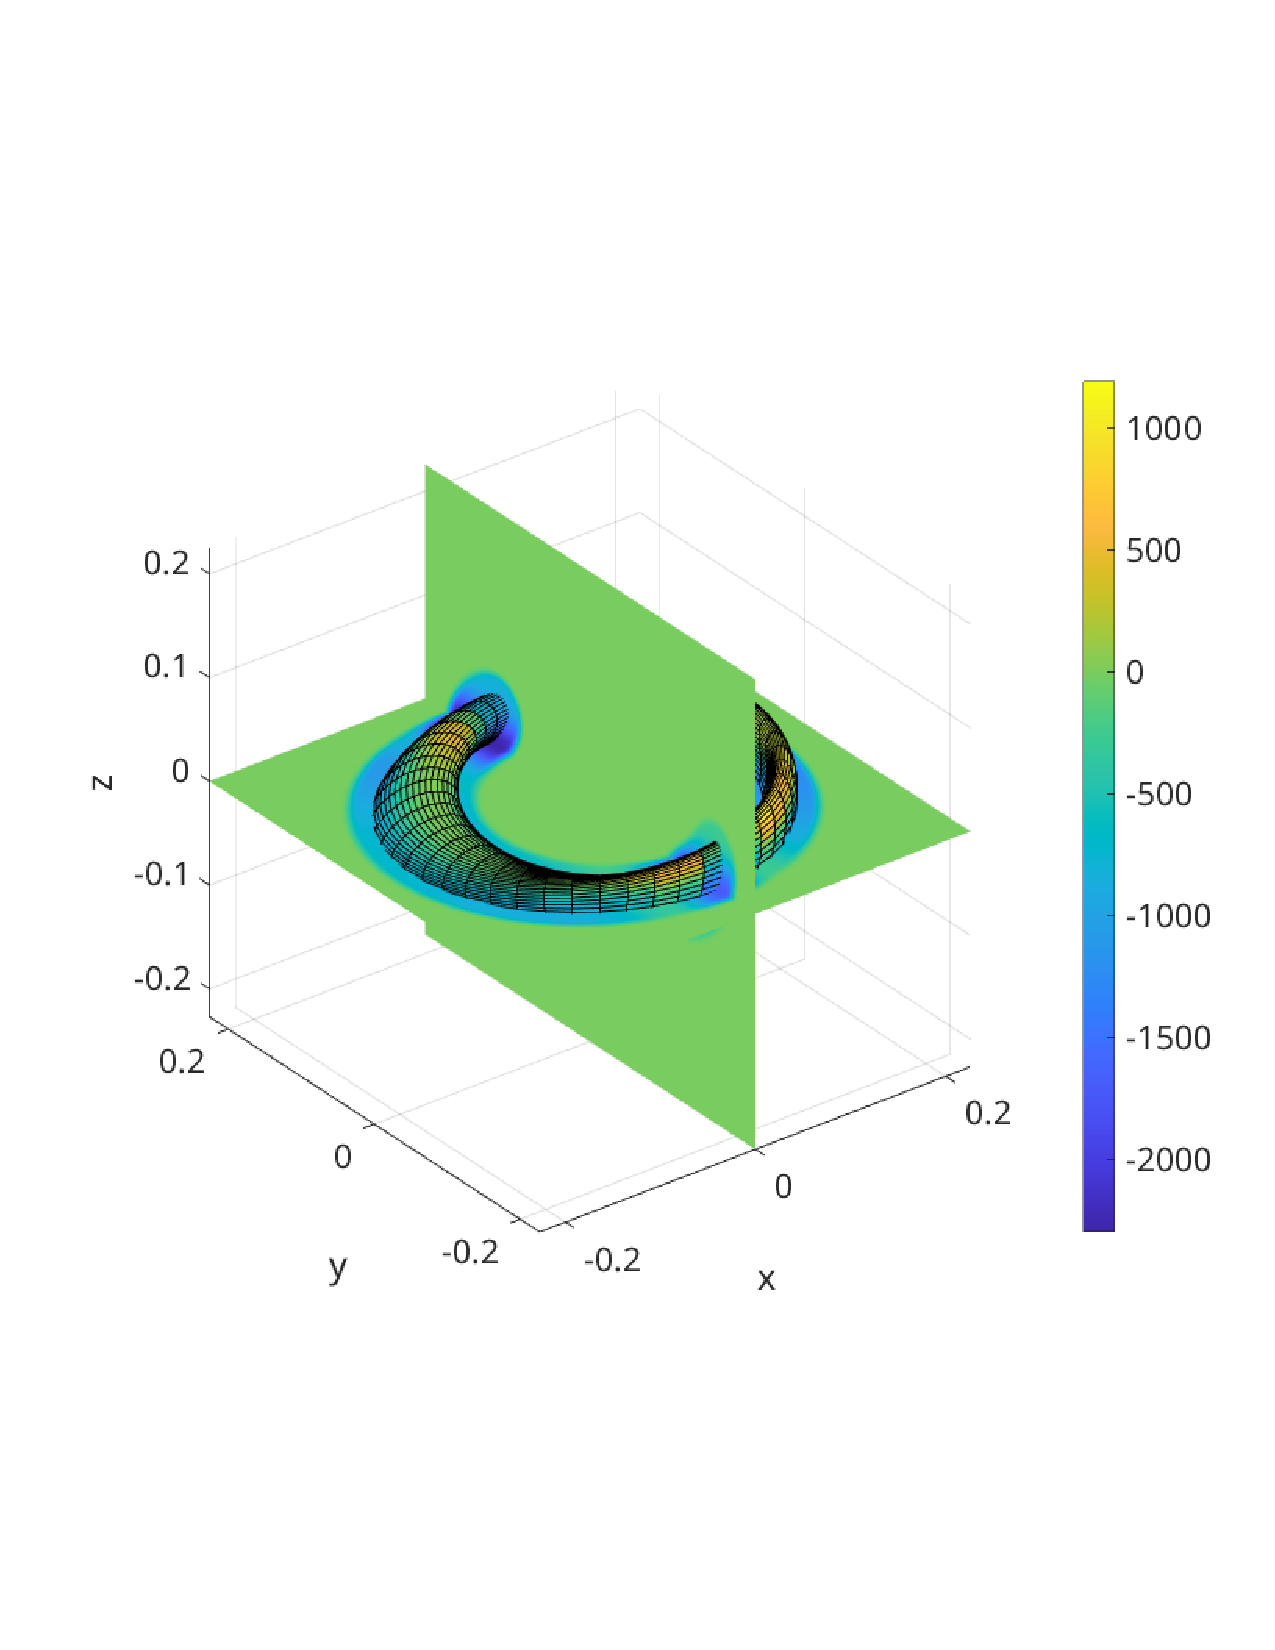
\includegraphics[trim={0cm 7cm 1cm 6cm},clip,width=\linewidth,height=0.65\textheight,keepaspectratio]{example23dfe.pdf}

\vspace{1mm}
\footnotesize Surface $\Gamma_5$, right-hand side $f_5$, and slices of its eighth-order EFJ extension $f_5^e$.
\end{column}
\begin{column}{0.49\textwidth}
\centering
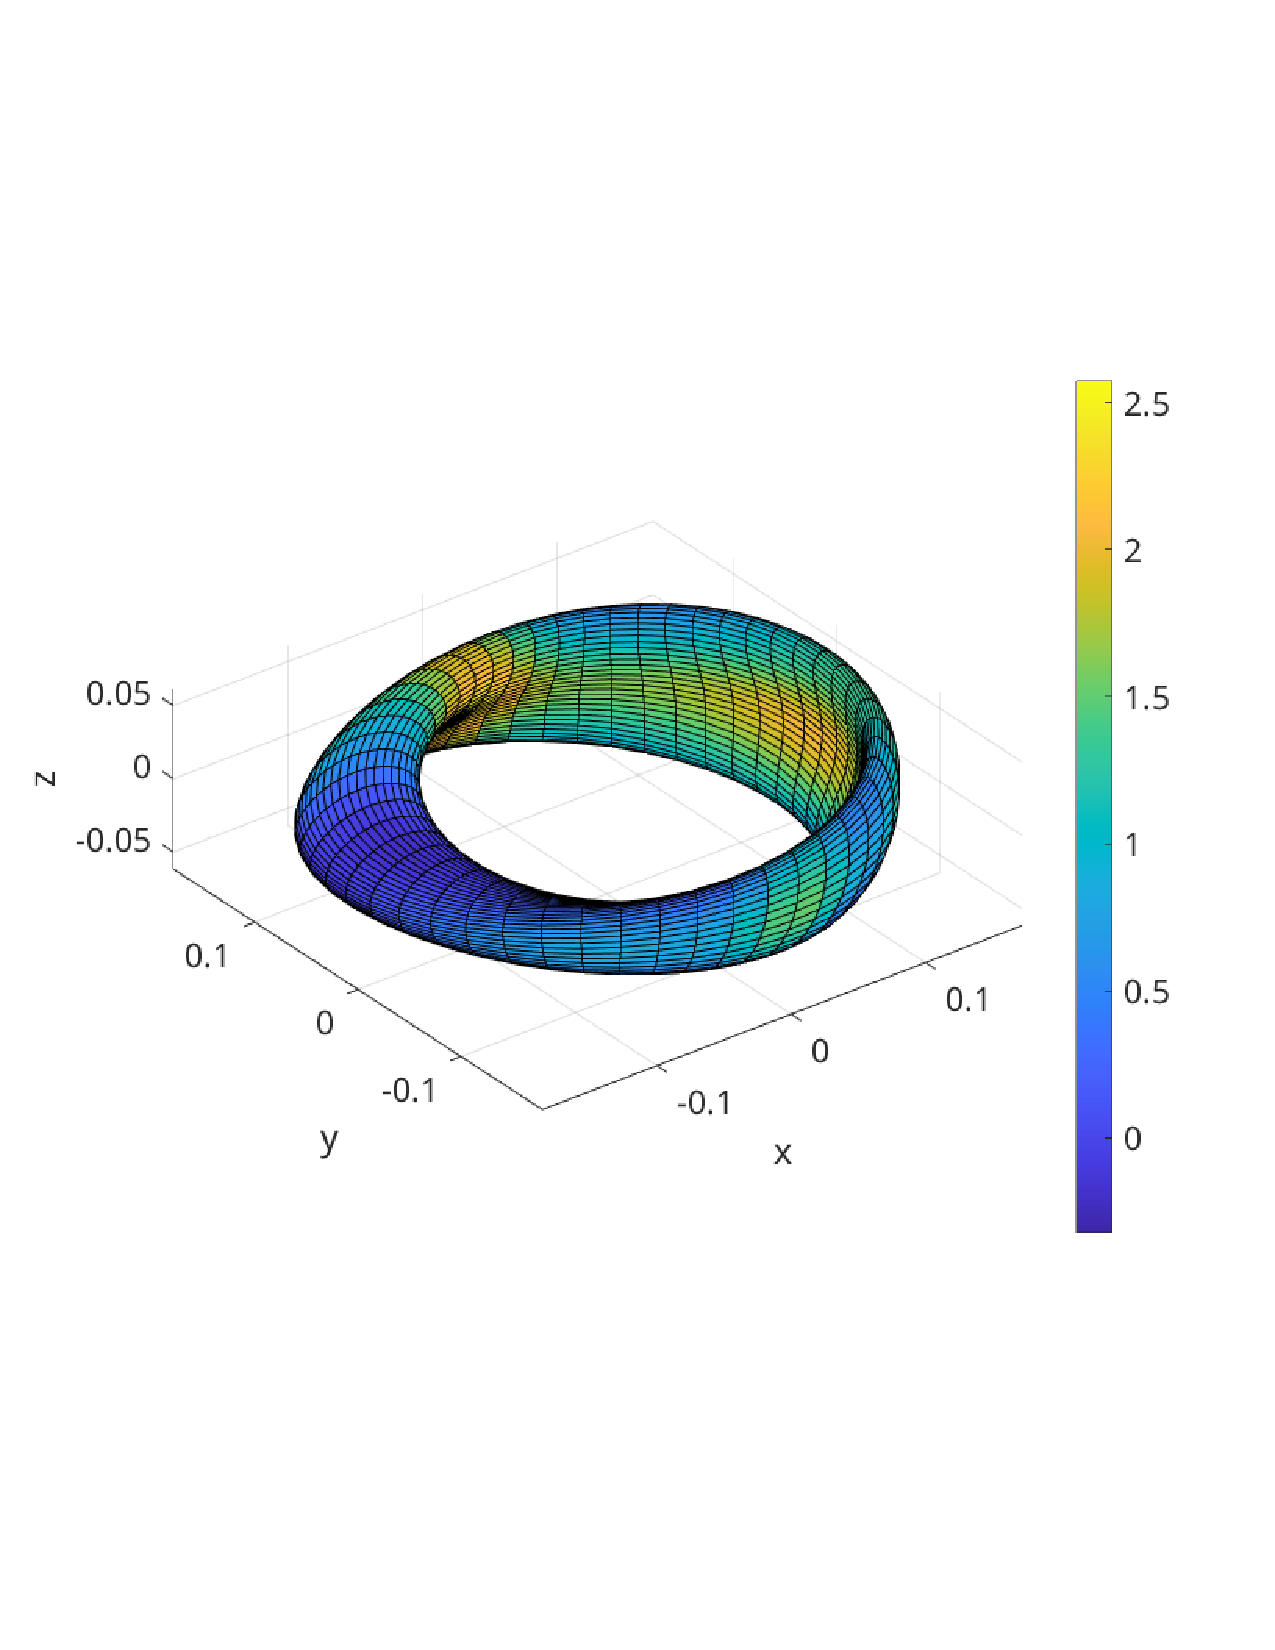
\includegraphics[trim={0cm 8cm 1cm 6cm},clip,width=\linewidth,height=0.65\textheight,keepaspectratio]{example23dsol.pdf}

\vspace{1mm}
\footnotesize Dirichlet boundary data $g_5$ on $\Gamma_5$.
\end{column}
\end{columns}
\end{frame}

%================================================================
\begin{frame}{3D timing example}
\centering
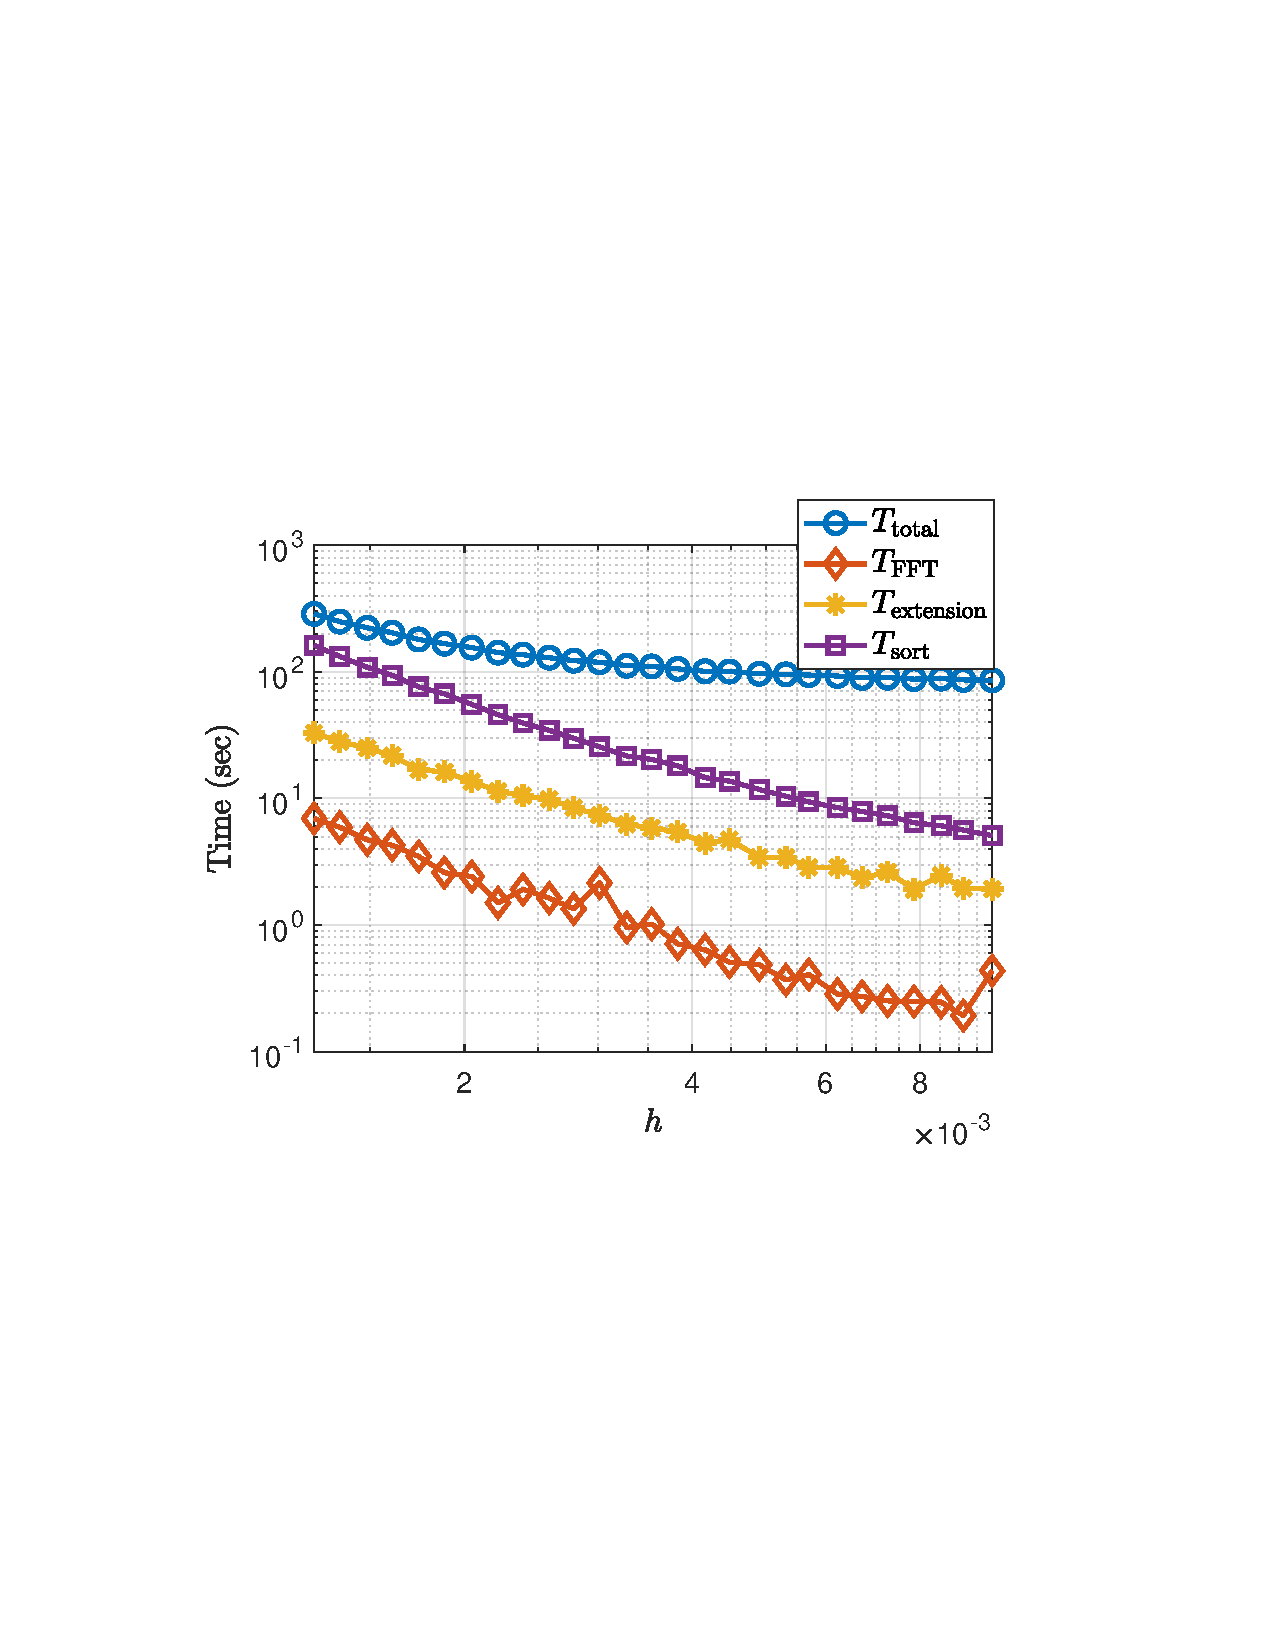
\includegraphics[trim={98pt 242pt 129pt 239pt},clip,height=0.72\textheight]{example23dtimings.pdf}

\vspace{1mm}
\scriptsize Function extension and sorting remain small compared with FFT-scale work.
\end{frame}

%================================================================
\begin{frame}{AAA comparison in two dimensions}
\small
For the first two-dimensional example, we compare the EFJ extension with AAA.

\vspace{2mm}
\begin{itemize}
  \item For each $\theta$, AAA produces a rational function $R_\theta$.
  \item The functions $R_\theta$ need not depend continuously on $\theta$.
  \item Smoothness of the extension in all variables is needed by the PDE solver.
\end{itemize}

\vfill
\footnotesize
Y. Nakatsukasa, O. S\`ete, and L. N. Trefethen,
\emph{The AAA algorithm for rational approximation},
\emph{SIAM Journal on Scientific Computing}, 40(3) (2018), A1494--A1522.
\end{frame}

%================================================================
\begin{frame}{AAA: PDE error and timing}
\begin{columns}[T,totalwidth=\textwidth]
\begin{column}{0.49\textwidth}
\centering
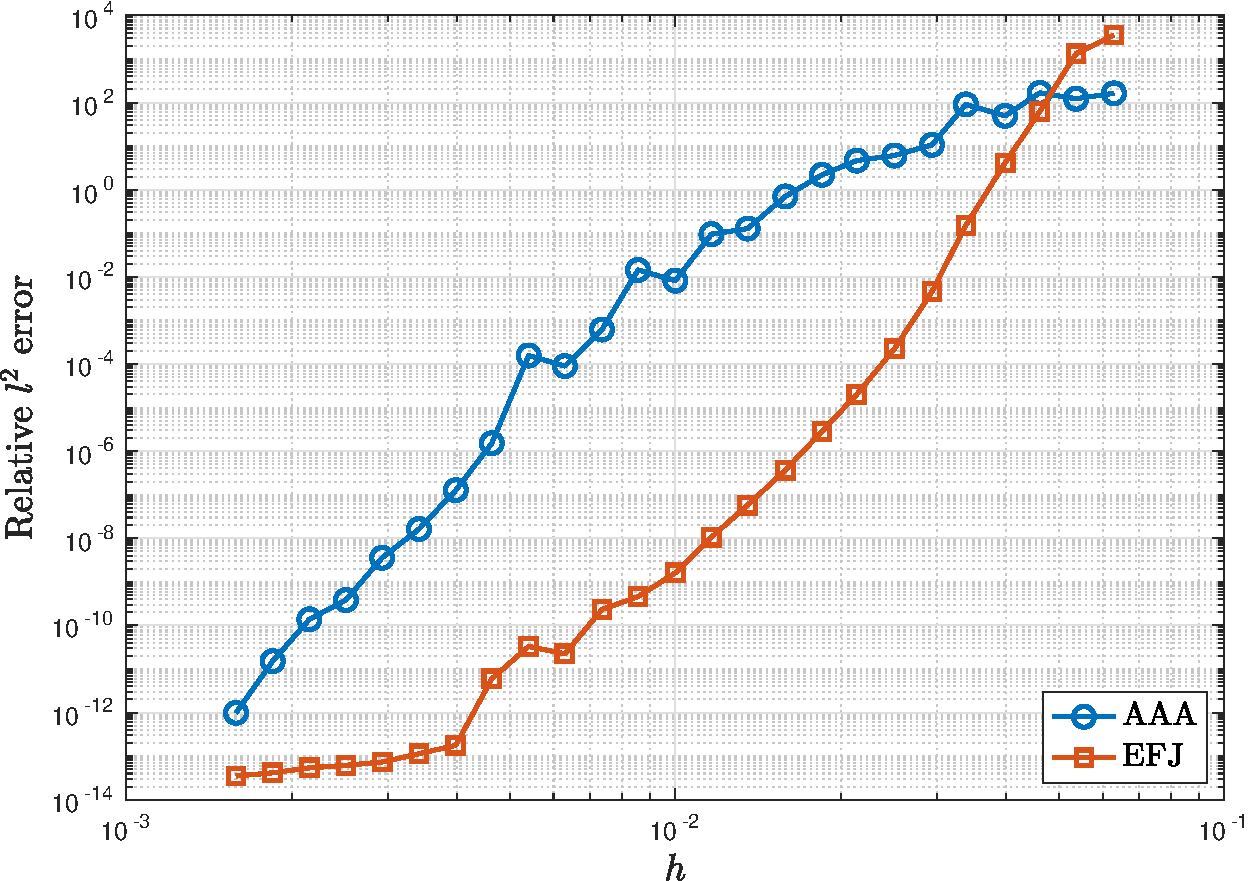
\includegraphics[width=\linewidth]{aaa_convergenceorder_new.pdf}

\vspace{1mm}
\footnotesize PDE error. The EFJ curve is our extension scheme.
\end{column}
\begin{column}{0.49\textwidth}
\centering
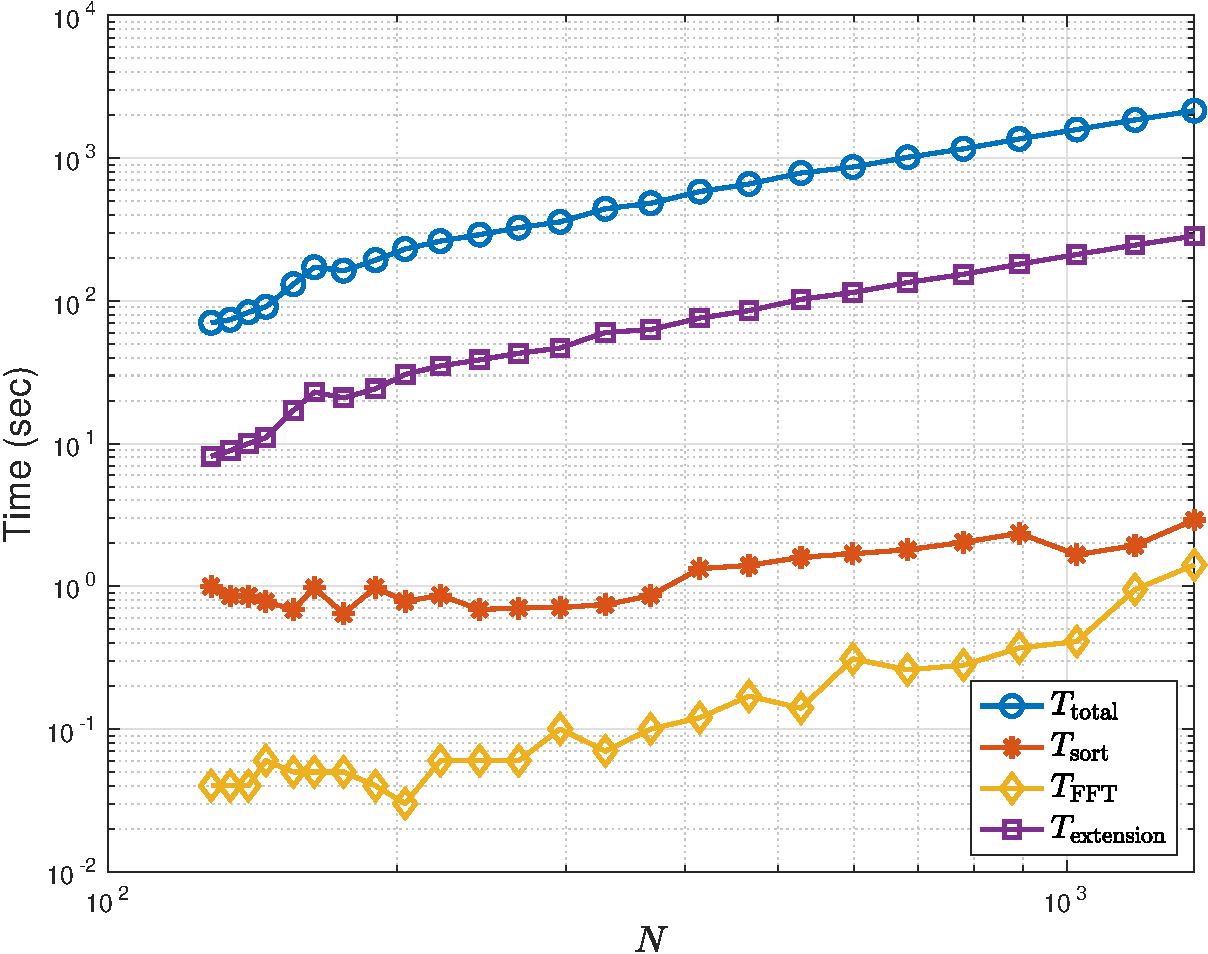
\includegraphics[width=\linewidth]{circle_timing_aaa_new.pdf}

\vspace{1mm}
\footnotesize Timing when AAA is used for extension.
\end{column}
\end{columns}
\end{frame}

%================================================================
\begin{frame}{Power spectra at $r=1.005$}
\begin{columns}[T,totalwidth=\textwidth]
\begin{column}{0.49\textwidth}
\centering
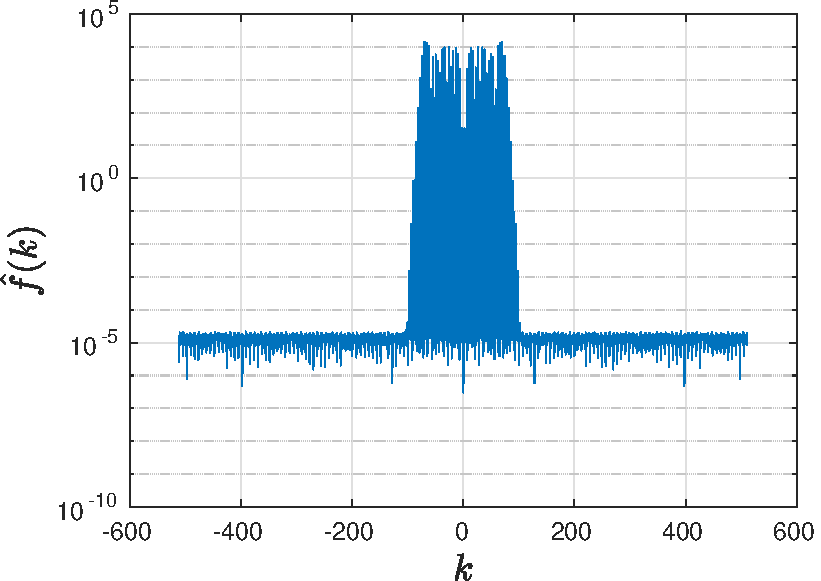
\includegraphics[width=\linewidth]{aaa1005ps.pdf}

\footnotesize AAA extension
\end{column}
\begin{column}{0.49\textwidth}
\centering
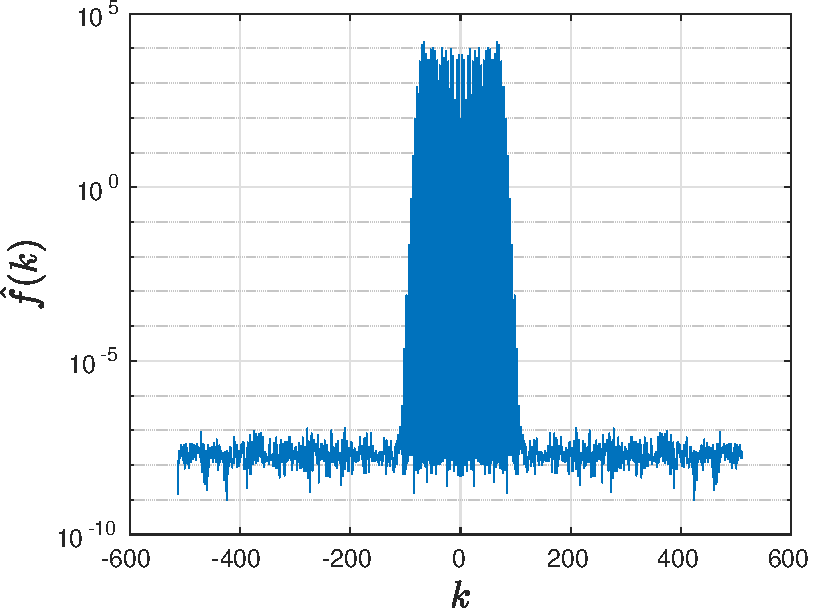
\includegraphics[width=\linewidth]{efj1005ps.pdf}

\footnotesize EFJ extension
\end{column}
\end{columns}
\end{frame}

%================================================================
\begin{frame}{Power spectra at $r=1.035$}
\begin{columns}[T,totalwidth=\textwidth]
\begin{column}{0.49\textwidth}
\centering
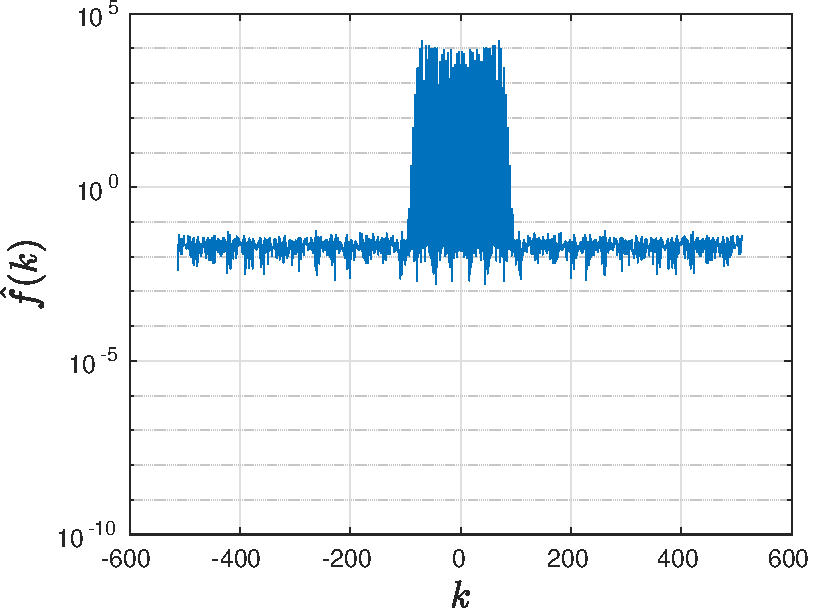
\includegraphics[width=\linewidth]{aaa1035ps.pdf}

\footnotesize AAA extension
\end{column}
\begin{column}{0.49\textwidth}
\centering
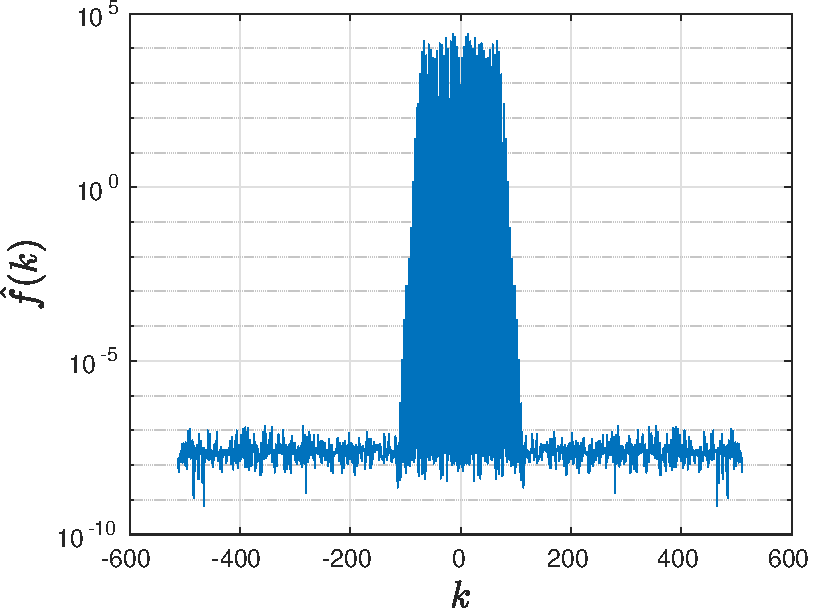
\includegraphics[width=\linewidth]{efj1035ps.pdf}

\footnotesize EFJ extension
\end{column}
\end{columns}
\end{frame}

%================================================================
\begin{frame}{Power spectra at $r=1.065$}
\begin{columns}[T,totalwidth=\textwidth]
\begin{column}{0.49\textwidth}
\centering
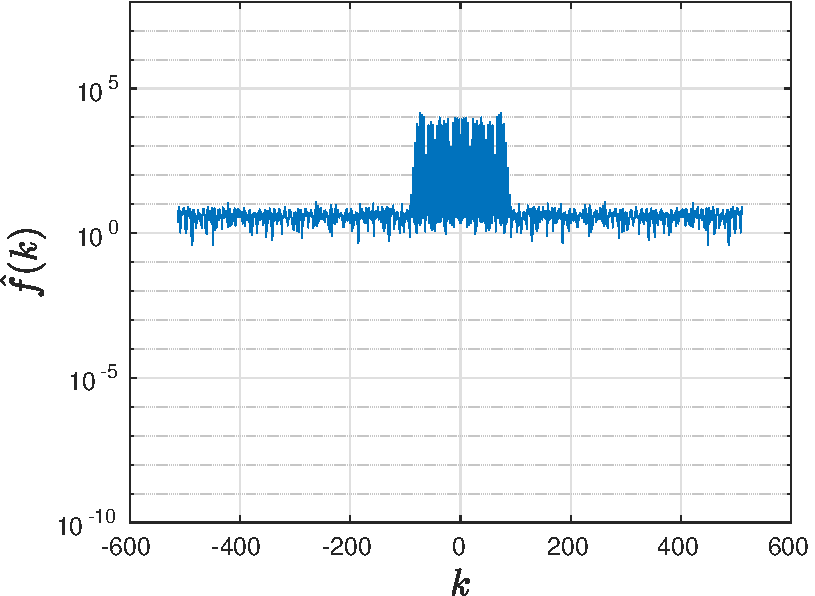
\includegraphics[width=\linewidth]{aaa1065ps.pdf}

\footnotesize AAA extension
\end{column}
\begin{column}{0.49\textwidth}
\centering
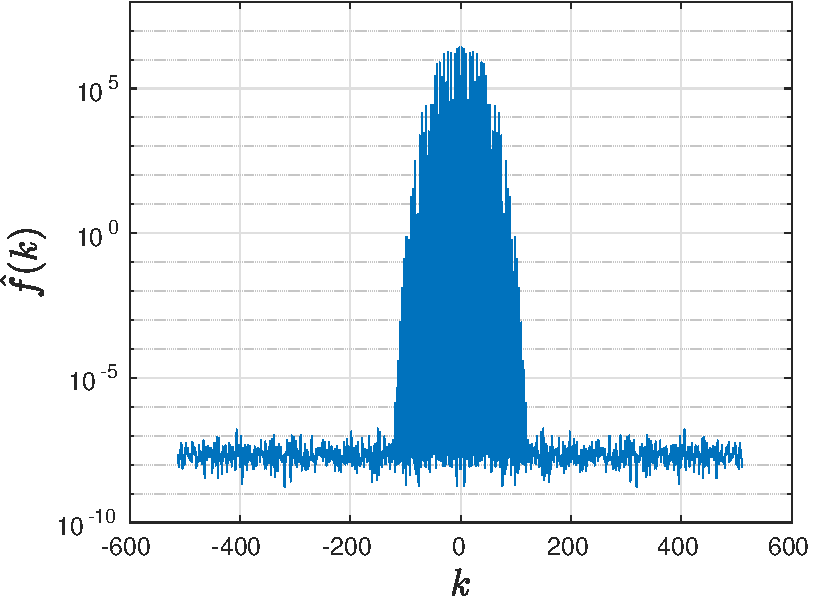
\includegraphics[width=\linewidth]{efj1065ps.pdf}

\footnotesize EFJ extension
\end{column}
\end{columns}
\end{frame}

%================================================================
\begin{frame}{Function-extension summary}
\small
\begin{enumerate}
  \item Extend exterior values along normals.
  \item Match normal derivatives through order $n$.
  \item The weights are Lagrange basis values at $-1$.
  \item Chebyshev nodes minimize the $\ell^1$ norm of the weights.
  \item A smooth window rolls the extension off for FFT use.
  \item The FFT particular solution is completed by a BIE correction.
\end{enumerate}
\end{frame}

%================================================================
\begin{frame}{References}
\scriptsize
\begin{itemize}
  \item F. Vico, L. Greengard, and M. Ferrando, \emph{Fast convolution with free-space Green's functions}, \emph{Journal of Computational Physics}, 323 (2016), 191--203.
  \item R. T. Seeley, \emph{Extension of $C^\infty$ functions defined in a half space}, \emph{Proceedings of the American Mathematical Society}, 15 (1964), 625--626.
  \item C. L. Epstein, F. Fryklund, and S. Jiang, \emph{An accurate and efficient scheme for function extension on smooth domains}, \emph{SIAM Journal on Numerical Analysis}, 63(4) (2025), 1427--1453.
  \item Y. Nakatsukasa, O. S\`ete, and L. N. Trefethen, \emph{The AAA algorithm for rational approximation}, \emph{SIAM Journal on Scientific Computing}, 40(3) (2018), A1494--A1522.
\end{itemize}
\end{frame}

\end{document}
